\documentclass[11pt]{article}
\usepackage[T1]{fontenc}
\usepackage{lmodern}
\usepackage[margin=1in,headheight=15pt]{geometry}
\usepackage{amsmath,amssymb,amsthm,mathtools}
\usepackage{microtype,booktabs,longtable,array,enumitem}
\usepackage{xcolor,graphicx,xurl,fancyhdr,placeins}
\definecolor{ink}{HTML}{183B50}
\definecolor{teal}{HTML}{258F8B}
\usepackage[colorlinks=true,linkcolor=ink,citecolor=ink,urlcolor=teal]{hyperref}
\usepackage{bookmark}
\hypersetup{pdftitle={Polylogarithm Continuation: Fractional Kernels, Cayley Quotients, and Joint Scaling Limits},pdfauthor={OpenAI-assisted research prepared for Vladimir Reshetnikov's ProveIt project}}
\pagestyle{fancy}\fancyhf{}
\fancyhead[L]{\small Polylogarithm continuation}
\fancyhead[R]{\small ProveIt research article}
\fancyfoot[C]{\thepage}
\setlength{\emergencystretch}{2em}
\setlength{\parskip}{3pt}
\setlist{itemsep=3pt,topsep=5pt}
\numberwithin{equation}{section}
\newtheorem{theorem}{Theorem}[section]
\newtheorem{lemma}[theorem]{Lemma}
\newtheorem{proposition}[theorem]{Proposition}
\newtheorem{corollary}[theorem]{Corollary}
\newtheorem{conjecture}[theorem]{Conjecture}
\theoremstyle{definition}\newtheorem{definition}[theorem]{Definition}
\theoremstyle{remark}\newtheorem{remark}[theorem]{Remark}
\DeclareMathOperator{\Li}{Li}
\newcommand{\E}{\mathbb E}
\newcommand{\dd}{\mathop{}\!\mathrm d}
\newcommand{\repo}{\texttt{ProveIt}}
\newcommand{\baseline}{\nolinkurl{28357e8ca63dd78327db91d9be239d75e4462879}}
\newcommand{\codefile}[1]{\nolinkurl{#1}}
\begin{document}
\hypersetup{pageanchor=false}
\begin{titlepage}
\vspace*{0.8cm}
{\color{teal}\large RESEARCH CONTINUATION\par}
\vspace{0.55cm}
{\color{ink}\LARGE\bfseries Polylogarithm Continuation\par}
\vspace{0.3cm}
{\color{ink}\Large Fractional Kernels, Cayley Quotients,\\[3pt]
and Joint Scaling Limits\par}
\vspace{0.75cm}
{\large Prepared for Vladimir Reshetnikov's \repo\ project\par}
\vspace{0.12cm}
{OpenAI-assisted mathematical research article\par}
{10 October 2026 (UTC)\par}
\vspace{0.8cm}
\begin{abstract}
We continue the signed-kernel, level-four relation, Stieltjes--Lerch zero,
and reflected log-gamma programmes in the \repo\ manuscript. For
$H_{n-1}^{(b)}/n^a$, we classify exactly the nonnegative outer orders and
positive inner orders admitting a finite signed Hausdorff moment measure.
The boundary contains positive endpoint atoms. The classification yields
complex nonvanishing, unique angular zeros, one-sided Euler enclosures,
and power-law or exponential atom-formation scales.

We prove the sign of the first nonconstant coefficient in the existing
normalized-radius conjecture for its full proposed range, including a
unique fractional-order threshold. An exact interval certificate proves
the emergence of a strict radial maximum below that threshold and,
at another inner order, a strict radial minimum above it.
For the derivative family with
$n=k+r$, an angular Cauchy estimate yields a complete Bessel expansion
uniform in the entire Lerch parameter interval. Its simple positive
Bessel branches move only exponentially under Lerch deformation. A
separate theorem gives the complete small-parameter positive-zero count
for every fixed pair of indices.

For reflected log-gamma moments, the critical scale
$n=(m+1)(\log m+c)$ has a nontrivial limiting factor
$\exp((\zeta(2)/(2\gamma)-\gamma)e^{-c})$; we prove the first uniform
correction. Finally, the full shuffle ideal generated by convergent
Cayley symmetry has an exactly determined polynomial quotient, Hilbert
series, conjugation character, and coefficient asymptotics. An explicit
all-index high-depth identity includes a 96-term expression for $S_6$.
The conjectured shorter depth-two reduction remains open.

Analytic proofs, finite rational certificates, symbolic coefficient
generation, and floating-point diagnostics are identified separately.
The accompanying package includes all source, reproducible verification,
integration notes, and a focused programme of further research.
\end{abstract}
\vfill
\noindent\small\textbf{Source snapshot.} \baseline.\\
\textbf{Status.} Ordinary mathematical proofs and reproducible exact
certificates; not proof-assistant verified or externally refereed.
Claims of newness refer to the inspected repository and reports.
\end{titlepage}
\hypersetup{pageanchor=true}
\pagenumbering{roman}
\tableofcontents
\clearpage
\pagenumbering{arabic}
\section{Scope, source snapshot, and result map}
\label{sec:scope}

The source manuscript is Vladimir Reshetnikov's \repo\ project,
under \codefile{Analysis/Polylogarithms/docs/manuscript}. We pinned the
working branch to commit \baseline\ and inspected its chapter sources,
editorial ledger, and the relevant pending research reports
\cite{ProveIt,AngularBaseline,LerchBaseline,CayleyBaseline}.
This matters mathematically: several older reports call $S_4$ a conjecture,
whereas the canonical manuscript now contains an exact proof. Its
specified level-four product-matrix rank conjecture is also already
proved. The $S_6$ depth-two identity is still conjectural, and an earlier
frozen $S_8$ search vector has already been rigorously refuted. None of
those completed results is counted here as a new theorem.

The present work concentrates on places where the existing hypotheses
leave a real mathematical boundary: outer orders below one, simultaneous
growth of asymptotic indices, and the difference between a set of
linear symmetry rows and its multiplicative closure. These boundaries
lead to the principal results in Table~\ref{tab:results}.

\begin{table}[htbp]
\centering\small
\begin{tabular}{@{}p{0.25\linewidth}p{0.67\linewidth}@{}}
\toprule
Result & Precise advance\\
\midrule
Sharp finite-measure domain & A necessary and sufficient condition for
$H_{n-1}^{(b)}/n^a$ to have a finite signed moment measure; explicit
interior densities and critical atoms
(Theorem~\ref{subunit:thm:domain}).\\[5pt]
Complex and angular zeros & Nonvanishing on the principal slit plane and
one simple imaginary-part zero on each open upper arc throughout the
full measure domain (Theorem~\ref{subunit:thm:zerofree}).\\[5pt]
Endpoint scales & Two power laws, an exponential logarithmic corner,
weak limits, and a sharp divergent signed-mass scale
(Theorem~\ref{subunit:thm:boundarylayer} and
Proposition~\ref{subunit:prop:otheredges}).\\[5pt]
Existing radial conjecture & The exact sign of its quadratic radial
coefficient for every real $a\ge2,b>0$, its $a=1$ boundary, and a
unique fractional threshold (Theorem~\ref{thm:radius-local-sign});
proved local maxima and minima at two certified inner orders
(Theorems~\ref{turn:thm:maximum} and \ref{turn:thm:minimum}).\\[5pt]
Adjacent-index zeros & A complete Bessel expansion for $n=k+r$, every
fixed integer $r$, uniform in $0\le\rho\le1$, with explicit zero
coefficients and exponential deformation bounds
(Theorems~\ref{bessel:thm:profile}--\ref{bessel:thm:zeros}).\\[5pt]
Small Lerch parameter & Complete positive-zero counts and central
Puiseux branches for every fixed $(n,k)$
(Theorem~\ref{unfold:thm:count}).\\[5pt]
Growing reflected moments & A uniform transition at
$n=(m+1)(\log m+c)$, its first correction and lattice location
(Theorem~\ref{thm:gamma-transition}).\\[5pt]
Cayley quotient and identities & Exact all-weight raw ranks and
shuffle-ideal Hilbert characters; a proved explicit family containing
$S_6$ (Theorems~\ref{cayley:thm:raw}--\ref{cayley:thm:ideal} and
Proposition~\ref{cayley:prop:harmonic}).\\
\bottomrule
\end{tabular}
\caption{Theorem-level advances relative to the inspected source.
Finite computations audit these results; their all-parameter statements
are established by the written proofs.}
\label{tab:results}
\end{table}

\subsection{Relation to established mathematics}
The regularized Hurwitz and digamma integrals used below are classical
\cite{DLMFhurwitz,DLMFdigamma}. The Bessel limit is proved here directly
from a finite elementary-symmetric product; the Bessel series and simple
positive zeros are classical \cite{DLMFbessel}. Its form is reminiscent
of Mehler--Heine limits, but no identification of these coefficient
polynomials with a classical orthogonal family is assumed.
The shuffle polynomial theorem is due to the classical work of Radford
and Melan\c{c}on--Reutenauer
\cite{cayley:radford,cayley:melancon-reutenauer}.
The Cayley transformation itself is inherited from the manuscript's
convergent octahedral argument; it is not introduced here as a new
change of variables. The broader use of octahedral symmetry at level
four has a precedent in Zhao \cite{ZhaoOctahedral}.

Reflected products of powers of $\log\Gamma$ were studied by
Amdeberhan, Coffey, Espinosa, Koutschan, Manna and Moll
\cite{ACEKMM}. In particular, the moments, their reflection symmetry,
and elementary identities obtained from Euler's reflection formula are
not new. Our contribution is the joint growth regime and its controlled
correction. Targeted primary-source research supports these attributions;
it does not establish exhaustive historical priority for every new
deduction in this article.

\section{Conventions and inherited analytic framework}
\label{sec:conventions}

For real $b>0$, let
\[
 H_N^{(b)}=\sum_{j=1}^N j^{-b},\qquad H_0^{(b)}=0,
 \qquad H_N=H_N^{(1)}.
\]
We use decreasing series indices and the outer-first convention
\[
 \Li_{s_1,\ldots,s_d}(z_1,\ldots,z_d)
 =\sum_{n_1>\cdots>n_d\ge1}
 \frac{z_1^{n_1}\cdots z_d^{n_d}}
 {n_1^{s_1}\cdots n_d^{s_d}}
\]
where convergent, followed by the stated analytic continuation.
In particular,
\[
 F_{a,b}(z)=\Li_{a,b}(z,1)
 =\sum_{n\ge1}\frac{H_{n-1}^{(b)}}{n^a}z^n,
 \qquad |z|<1.
\]
The slit plane is $\mathbb C\setminus[1,\infty)$, and logarithms
there are continued from the disk. Later, $g_{a,b}=\Im F_{a,b}(i)$
denotes a Gaussian double, $\beta(s)=\sum_{j\ge0}(-1)^j/(2j+1)^s$
is the Dirichlet beta function, and
\[
 S_p=\sum_{j\ge0}\frac{(-1)^jH_j}{(2j+1)^p}.
\]
The last sum is absolute for integers $p>1$ and converges conditionally
for $p=1$. Throughout, $\gamma$ without an index is Euler's constant.

The Stieltjes constants use
\[
 \zeta(s,a)=\frac1{s-1}
  +\sum_{n\ge0}\frac{(-1)^n\gamma_n(a)}{n!}(s-1)^n.
\]
A superscript $(k)$ on $\gamma_n$ means differentiation in $a$.
For $0\le\rho<1$ set
\[
 \ell_n(\rho,a)=\sum_{j\ge0}\frac{\rho^j\log^n(a+j)}{a+j},
 \qquad
 \mathcal D_{n,k}^{\rho}(a)=\partial_a^k\ell_n(\rho,a),
 \qquad k\ge1,
\]
and define $\mathcal D_{n,k}^{1}(a)=\gamma_n^{(k)}(a)$.
Only the differentiated family is unified at $\rho=1$; the series
defining $\ell_n$ generally diverges there. The sign-normalized family is
\[
 F_{n,k}^{\rho}(a)=(-1)^{n+k}\mathcal D_{n,k}^{\rho}(a).
\]
The same symbol $F$ with different indices is conventional in the
source: $F_{a,b}(z)$ is a double polylogarithm, while
$F_{n,k}^{\rho}(a)$ is the Stieltjes--Lerch derivative family.
The radius $\rho$ in the angular sections and the Lerch parameter
$\rho$ in the zero sections are separate variables.

The master coefficient formula, reproduced in
\eqref{bessel:eq:shift}, follows from differentiating
$(a+j)^{-s}$ in $a$ and extracting the coefficient of $s-1$.
For $k\ge1$ its shift series and every fixed number of $a$
derivatives converge locally uniformly for $a>0$, uniformly in
$0\le\rho\le1$. The bound is a fixed power of
$\log(a+j)$ divided by $(a+j)^{k+1}$.
This convergence justifies the classical endpoint without assigning
a value to the divergent undifferentiated series.

All finite signed measures in the article are real measures of finite
total variation. Weak convergence means convergence against every
continuous function on $[0,1]$. Big-$O$ constants may depend on fixed
indices and fixed compact parameter sets; every claimed uniformity is
stated explicitly.

% Research component, 2026-10-10. Parent may adapt labels and bibliography.
% Baseline: 28357e8ca63dd78327db91d9be239d75e4462879.
\section{The sharp signed-moment threshold for subunit orders}
\label{subunit:sec:main}

The earlier angular-zero continuation \cite{AngularBaseline} extends the signed Mellin kernel
from integer outer order to real $a\geq1$. The restriction $a\geq1$ is
not the actual boundary of this method. The correct boundary is
$a+b=1$ when $0<b<1$. At that boundary a density becomes a measure with
a positive atom at one. The atom must be retained: substituting zero
for a vanishing reciprocal Gamma factor would lose its entire mass.

Write
\[
 A_n(a,b)=\frac{H_{n-1}^{(b)}}{n^a},\qquad
 F_{a,b}(z)=\sum_{n\geq1}A_n(a,b)z^n\quad(|z|<1).
\]
We permit $a=0$ to state the sharp endpoint. Throughout $b>0$.

\begin{theorem}[Exact finite-measure domain]
\label{subunit:thm:domain}
For $a\geq0$ and $b>0$, a finite real signed measure $\nu_{a,b}$ on
$[0,1]$ satisfying
\begin{equation}\label{subunit:eq:moments}
 \int_{[0,1]}u^{n-1}\,d\nu_{a,b}(u)=A_n(a,b)
 \qquad(n\geq1)
\end{equation}
exists if and only if
\begin{equation}\label{subunit:eq:domain}
 (a>0\ \hbox{and}\ a+b\geq1)
 \quad\hbox{or}\quad(a=0\ \hbox{and}\ b>1).
\end{equation}
It is unique and has total mass zero. More precisely:
\begin{enumerate}
\item If $a>0$ and $a+b>1$, it has an integrable density
      $\kappa_{a,b}(u)$ with exactly one strict sign change, from
      negative to positive as $u$ increases, at a point $r_{a,b}\in(0,1)$.
\item If $0<b<1$ and $a=1-b$, then
      $\nu_{a,b}=(1-b)^{-1}\delta_1+\kappa_{a,b}(u)\,du$,
      where $\kappa_{a,b}(u)<0$ throughout $(0,1)$.
\item If $a=0$ and $b>1$, then
      $\nu_{0,b}=\zeta(b)\delta_1+\kappa_{0,b}(u)\,du$,
      where $\kappa_{0,b}(u)<0$ throughout $(0,1)$.
\end{enumerate}
In the two atomic cases all positive mass is at one and all negative
mass is in $(0,1)$. Outside \eqref{subunit:eq:domain}, not even a
finite signed measure with arbitrarily many sign changes can satisfy
\eqref{subunit:eq:moments}.
\end{theorem}

\begin{figure}[tbp]
\centering
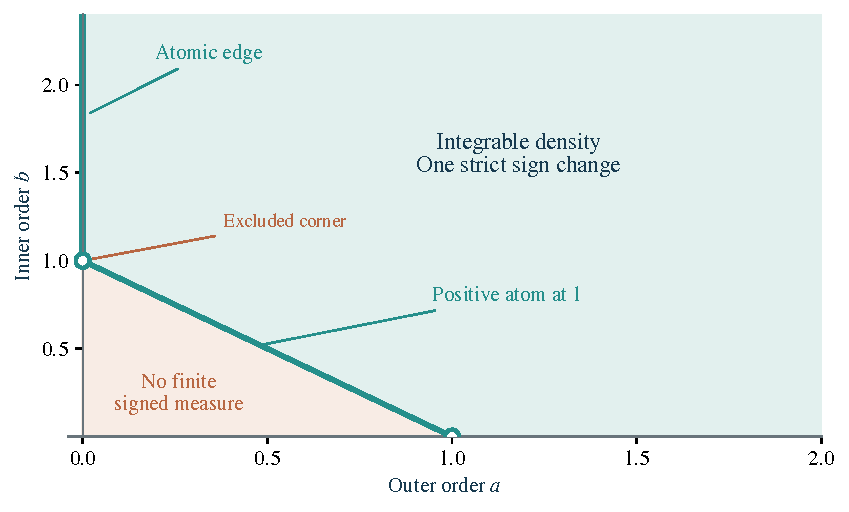
\includegraphics[width=0.8\linewidth]{figures/signed_measure_domain.pdf}
\caption{The exact finite signed-measure domain for $a\ge0,b>0$.
The teal edges carry a positive atom at one. The point $(0,1)$ is
excluded, and the horizontal axis $b=0$ is outside the stated domain.
The absence of a finite measure below the diagonal does not assert
the presence of a complex zero.}
\label{fig:measure-domain}
\end{figure}

\subsection{A regularized positive kernel}

Set
\begin{equation}\label{subunit:eq:q}
 q(t)=\frac1{1-e^{-t}}-\frac1t,\qquad t>0.
\end{equation}
The elementary identities
\[
 q(t)=\frac12+\frac12\coth(t/2)-\frac1t,
 \qquad
 q'(t)=\frac1{t^2}-\frac1{4\sinh^2(t/2)}>0
\]
give $1/2<q(t)<1$, because $\sinh(t/2)>t/2$ and the endpoint
limits are $1/2$ and $1$. In particular $q$ is positive, bounded and
strictly increasing. Also $q(t)=1/2+O(t)$ as $t\downarrow0$.

The classical Hurwitz integral and one elementary subtraction give
\begin{equation}\label{subunit:eq:hurwitz}
 \zeta(b,x)=\frac{x^{1-b}}{b-1}
 +\frac1{\Gamma(b)}\int_0^\infty
              e^{-xt}t^{b-1}q(t)\,dt,
 \qquad x>0,\ b>0,\ b\ne1.
\end{equation}
For $b>1$ this is obtained by splitting $1/(1-e^{-t})=1/t+q(t)$
in the usual Gamma integral. The integral involving $q$ is holomorphic
for $\Re b>0$, so the identity theorem extends the same formula to
$0<b<1$. This is analytic continuation of an absolutely convergent
regularized integral, not subtraction of two divergent real integrals.
The standard starting integral and recurrence are DLMF
25.11.25 and 25.11.4 \cite{DLMFhurwitz}. For $b=1$ the corresponding formula is
\begin{equation}\label{subunit:eq:digamma}
 \psi(x)=\log x-\int_0^\infty e^{-xt}q(t)\,dt,
\end{equation}
which is DLMF 5.9.13 \cite{DLMFdigamma} and also follows by taking the finite part of
\eqref{subunit:eq:hurwitz} at $b=1$.

For $0<b<1$, we shall use $\zeta(b)<0$. Indeed the alternating
Dirichlet series $\eta(b)$ is positive, while
$\eta(b)=(1-2^{1-b})\zeta(b)$ and $1-2^{1-b}<0$.

\subsection{Explicit densities and their Laplace transforms}

Put $T=-\log u$ and $K_{a,b}(T)=\kappa_{a,b}(e^{-T})$. For
$a>0$, $a+b>1$ and $b\ne1$, define
\begin{align}\label{subunit:eq:generalK}
 K_{a,b}(T)={}&\frac{\zeta(b)T^{a-1}}{\Gamma(a)}
 -\frac{T^{a+b-2}}{(b-1)\Gamma(a+b-1)}\notag\\
 &-\frac1{\Gamma(a)\Gamma(b)}
    \int_0^T(T-t)^{a-1}t^{b-1}q(t)\,dt.
\end{align}
When $b>1$, an equivalent form is
\begin{equation}\label{subunit:eq:largeB}
 K_{a,b}(T)=\frac{\zeta(b)T^{a-1}}{\Gamma(a)}
 -\frac1{\Gamma(a)\Gamma(b)}
   \int_0^T\frac{(T-t)^{a-1}t^{b-1}}{1-e^{-t}}\,dt.
\end{equation}
At $b=1$, define
\begin{align}\label{subunit:eq:bOne}
 K_{a,1}(T)={}&\frac{T^{a-1}}{\Gamma(a)}
       \bigl(\gamma+\psi(a)-\log T\bigr)\notag\\
 &-\frac1{\Gamma(a)}\int_0^T(T-t)^{a-1}q(t)\,dt.
\end{align}
The Gamma factors and the term $\gamma+\psi(a)$ in this last formula
are essential; in particular it reduces at $a=1$ to
$K_{1,1}(T)=-\log(e^T-1)$, agreeing with the original signed kernel.

These functions are integrable against $e^{-T}\,dT$. At zero,
\eqref{subunit:eq:generalK} has only the integrable powers
$T^{a-1}$, $T^{a+b-2}$ and $O(T^{a+b-1})$; the logarithmic factor
in \eqref{subunit:eq:bOne} is likewise integrable for $a>0$.
At infinity all terms have at most polynomial times logarithmic growth.
For $b>1$, the integrability of the convolution in
\eqref{subunit:eq:largeB} at its lower endpoint uses $b>1$ explicitly.

By the Gamma integral and the convolution rule, the Laplace transform
of \eqref{subunit:eq:generalK} is
\begin{align*}
 \int_0^\infty e^{-nT}K_{a,b}(T)\,dT
  &=n^{-a}\left[\zeta(b)-\frac{n^{1-b}}{b-1}
     -\frac1{\Gamma(b)}\int_0^\infty
                         e^{-nt}t^{b-1}q(t)\,dt\right]\\
  &=n^{-a}\bigl(\zeta(b)-\zeta(b,n)\bigr)
   =\frac{H_{n-1}^{(b)}}{n^a}.
\end{align*}
Each convolution interchange is justified absolutely; $q$ is bounded
and the remaining factors have Gamma integrals. Formula
\eqref{subunit:eq:bOne} has Laplace transform
\[
 n^{-a}\left(\gamma+\log n-\int_0^\infty e^{-nt}q(t)\,dt\right)
 =n^{-a}(\gamma+\psi(n))=\frac{H_{n-1}}{n^a}.
\]
Here the Laplace transform of $T^{a-1}\log T$ is obtained by
differentiating the Gamma integral, justified by absolute integrability.
The substitution $u=e^{-T}$ changes $u^{n-1}\,du$ to
$e^{-nT}\,dT$, proving the desired moment normalization. In particular
$n=1$ gives total mass zero.

\subsection{The one-sign-change proof}

For $b>1$, divide \eqref{subunit:eq:largeB} by $T^{a-1}$ and
rescale $t=Tv$:
\[
 T^{1-a}K_{a,b}(T)=\frac{\zeta(b)}{\Gamma(a)}
 -\frac1{\Gamma(a)\Gamma(b)}
  \int_0^1(1-v)^{a-1}v^{b-1}\frac{T^b}{1-e^{-Tv}}\,dv.
\]
For fixed $v>0$, the logarithmic derivative of
$T^b/(1-e^{-Tv})$ is
\[
 \frac bT-\frac{v}{e^{Tv}-1}>\frac{b-1}{T}>0.
\]
Thus the rescaled density is strictly decreasing. Its limit at zero is
$\zeta(b)/\Gamma(a)>0$, and its limit at infinity is $-\infty$.
This proves one strict positive--negative crossing in the $T$ coordinate.

For $b=1$, the rescaled expression is
\[
 \Gamma(a)T^{1-a}K_{a,1}(T)
 =\gamma+\psi(a)-\log T
  -T\int_0^1(1-v)^{a-1}q(Tv)\,dv.
\]
It is strictly decreasing from $+\infty$ to $-\infty$, since $q$ is
positive and increasing. For $0<b<1$, instead divide by
$T^{a+b-2}$ to obtain
\begin{align}\label{subunit:eq:rescaledLowB}
 T^{2-a-b}K_{a,b}(T)={}&
 \frac1{(1-b)\Gamma(a+b-1)}
 +\frac{\zeta(b)}{\Gamma(a)}T^{1-b}\notag\\
 &-\frac{T}{\Gamma(a)\Gamma(b)}
   \int_0^1(1-v)^{a-1}v^{b-1}q(Tv)\,dv.
\end{align}
Now the first term is positive, the second is strictly decreasing
because $\zeta(b)<0$, and the final term is strictly decreasing because
$q$ is positive and increasing. The endpoint limits are a positive
constant and $-\infty$. Thus there is again exactly one strict crossing.
The derivatives of these rescaled expressions are strictly negative;
differentiation is dominated by the same integrable beta weights.
At a zero of $K$, multiplication by the positive rescaling factor does
not affect the sign of its derivative. Reversing $T=-\log u$ gives
the asserted negative--positive sign change and a strictly positive
$u$ derivative at its unique crossing.

\subsection{The critical atom and the exact boundary}

Let $0<b<1$ and $a=1-b$. Replace the middle term of
\eqref{subunit:eq:generalK} by an atom of mass $(1-b)^{-1}$ at $u=1$,
and retain the density
\begin{equation}\label{subunit:eq:criticaldensity}
 K_{1-b,b}(T)=\frac{\zeta(b)T^{-b}}{\Gamma(1-b)}
 -\frac1{\Gamma(1-b)\Gamma(b)}
   \int_0^T(T-t)^{-b}t^{b-1}q(t)\,dt.
\end{equation}
Both terms are strictly negative and integrable against $e^{-T}\,dT$.
Its moments plus the atom are
\[
 \frac1{1-b}+n^{b-1}\left[\zeta(b)
   -\frac1{\Gamma(b)}\int_0^\infty e^{-nt}t^{b-1}q(t)\,dt\right]
 =\frac{H_{n-1}^{(b)}}{n^{1-b}},
\]
by \eqref{subunit:eq:hurwitz}. Thus the measure has total mass zero,
and its negative mass is exactly $(1-b)^{-1}$.

For $a=0$, $b>1$, the formula is especially simple:
\begin{equation}\label{subunit:eq:aZero}
 \nu_{0,b}=\zeta(b)\delta_1+K_{0,b}(-\log u)\,du,
 \qquad K_{0,b}(T)=-\frac{T^{b-1}}{\Gamma(b)(1-e^{-T})}.
\end{equation}
The ordinary Hurwitz integral gives its moments immediately. Its
negative mass is exactly $\zeta(b)$.

Every finite signed measure has bounded moments, since
$|\int u^{n-1}\,d\nu|\leq\|\nu\|_{\mathrm{TV}}$.
If $0<b<1$, elementary integral comparison gives
$H_{n-1}^{(b)}\sim n^{1-b}/(1-b)$, so the moments diverge to
infinity when $a+b<1$. If $a=0,b=1$, they diverge logarithmically.
These are exactly the excluded cases for $a\geq0,b>0$.
Finally, two finite signed measures with the same moments integrate
every polynomial equally; polynomial density in $C([0,1])$ makes the
measures identical. This proves Theorem~\ref{subunit:thm:domain}.

\section{Consequences for complex zeros and angular zeros}

\begin{theorem}[Nonvanishing throughout the finite-measure domain]
\label{subunit:thm:zerofree}
For all parameters in \eqref{subunit:eq:domain}, $F_{a,b}$ has an
analytic continuation to $\mathbb C\setminus[1,\infty)$ and has no
zero there except for its double zero at the origin. Every upper
open semicircle $z=\rho e^{i\theta}$, $0<\rho\leq1$, $0<\theta<\pi$,
has exactly one
simple zero of $\operatorname{Im}F_{a,b}(z)$, and it satisfies
\[
 \arccos\rho<\theta_{a,b}(\rho)<\frac\pi2.
\]
The imaginary part is positive below this angle and negative above
it; its angular derivative at the zero is strictly negative.
In the atomic cases, unit-circle values mean analytic continuation
or Abel boundary values: the original Fourier summands do not tend
to zero, so ordinary Fourier convergence is not asserted.
\end{theorem}

\begin{proof}
The signed transform
\[
 F_{a,b}(z)=z\int_{[0,1]}\frac{d\nu_{a,b}(u)}{1-zu}
\]
follows by geometric expansion in the disk and extends analytically
to the slit plane by uniform domination on compact sets. Let $r$ be
the crossing from Theorem~\ref{subunit:thm:domain}, or let $r=1$ in
the atomic cases. Zero mass gives
\begin{equation}\label{subunit:eq:factor}
 F_{a,b}(z)=\frac{z^2}{1-rz}P_{a,b}(z),\qquad
 P_{a,b}(z)=\int_{[0,1]}\frac{u-r}{1-zu}\,d\nu_{a,b}(u).
\end{equation}
The measure $(u-r)\,d\nu_{a,b}(u)$ is positive and nonzero, including
when $r=1$: its atom disappears but its density is strictly positive
on $(0,1)$. Consequently $\operatorname{Im}P_{a,b}(z)$ has the
strict sign of $\operatorname{Im}z$, while $P_{a,b}(x)>0$ for
$x<1$. Apart from the explicit $z^2$, the factor $(1-rz)^{-1}$ in
\eqref{subunit:eq:factor} is analytic and nonzero on the slit plane. Since $P_{a,b}(0)=A_2=2^{-a}$,
the zero at zero has multiplicity exactly two.

For angular zeros put
\[
 J_\rho(c)=\int_{[0,1]}\frac{d\nu(u)}{1-2\rho cu+\rho^2u^2},
 \qquad
 \operatorname{Im}F(\rho e^{i\theta})
       =\rho\sin\theta\,J_\rho(\cos\theta).
\]
The zero-mass one-crossing sign test holds for our atomic measures as
well: subtract the value of the test function at $r$, and use the
ordered supports of the two signs. It gives $J_\rho(0)<0$.
When $\rho<1$, the kernel at $c=\rho$ is strictly increasing in $u$,
so $J_\rho(\rho)>0$. When $\rho=1$ and the crossing is interior,
separate the two signs before expanding $(1-u)^{-2}$ to obtain
\[
 \lim_{c\uparrow1}J_1(c)
 =\int_{[0,1]}\frac{d\nu(u)}{(1-u)^2}
 =\sum_{n\geq1}n A_n>0,
\]
allowing $+\infty$. The negative part is supported away from one, so
this is the same justified monotone-limit argument as in the original
signed-kernel theorem. In the atomic cases the limiting signed
integral at $c=1$ need not be defined, and we do not use that display.
Instead the limit is $+\infty$ directly: the atom contributes
$M/[2(1-c)]$, and the negative density contributes
$o((1-c)^{-1})$. For the latter assertion, multiply its integral by
$1-c$ and use dominated convergence: the multiplier
$(1-c)/(1-2cu+u^2)$ is bounded by $1$ for $0\leq c<1$ and tends to zero for
every $u<1$. The negative density is integrable and has no atom at one.

For $c'>c$, the quotient of the two kernels has derivative
\[
 \frac{d}{du}\frac{1-2\rho cu+\rho^2u^2}
                         {1-2\rho c'u+\rho^2u^2}
 =\frac{2\rho(c'-c)(1-\rho^2u^2)}
       {(1-2\rho c'u+\rho^2u^2)^2}>0\quad(0<u<1).
\]
At any zero, apply the sign test to the signed measure obtained by
weighting $\nu$ with the positive kernel. It follows that $J_\rho$
is positive at every larger $c$ and negative at every smaller $c$;
this proves uniqueness and the signs. Finally its derivative at its
zero is positive, because the additional factor
$2\rho u/(1-2\rho cu+\rho^2u^2)$ is strictly increasing in $u$.
The angular derivative is therefore
$-\rho\sin^2\theta\,J_\rho'(\cos\theta)<0$.
\end{proof}

The theorem is sharp as a statement about finite signed moment
representations. It does not assert that nonvanishing fails below
$a+b=1$: the absence of this particular representation is not a
complex-zero counterexample. In fact the entire axis $a=0,b>0$ is zero-free away from the origin.
The geometric sum gives
\[
 F_{0,b}(z)=\frac{z\Li_b(z)}{1-z}
 =\frac{z^2}{1-z}\frac1{\Gamma(b)}
       \int_0^1\frac{(-\log u)^{b-1}}{1-zu}\,du.
\]
The last integral is a nonzero positive-measure transform on the slit
plane, by exactly the imaginary-part and real-axis argument used above.
Thus finite signed-moment representability and complex nonvanishing
have different parameter boundaries, already on this explicit axis.

\section{Formation of the endpoint atom}

\begin{theorem}[Boundary-layer scale and weak convergence]
\label{subunit:thm:boundarylayer}
Fix $0<b<1$, let $a=1-b+\varepsilon$ with $\varepsilon>0$, and
let $T_\varepsilon=-\log r_{a,b}$. Define
\[
 \tau_\varepsilon=
 \left(\frac{\Gamma(1-b+\varepsilon)}
 {(1-b)(-\zeta(b))\Gamma(\varepsilon)}\right)^{1/(1-b)}.
\]
Then, as $\varepsilon\downarrow0$,
\begin{equation}\label{subunit:eq:layerexact}
 T_\varepsilon=\tau_\varepsilon
 \left(1+O_b\left(\frac{\tau_\varepsilon}{\varepsilon}\right)\right),
 \qquad 0<T_\varepsilon<\tau_\varepsilon,
\end{equation}
and in particular
\begin{equation}\label{subunit:eq:layerleading}
 1-r_{1-b+\varepsilon,b}\sim
 \left(\frac{\Gamma(1-b)}{(1-b)(-\zeta(b))}
       \varepsilon\right)^{1/(1-b)}.
\end{equation}
The measures converge weakly to the critical measure in
Theorem~\ref{subunit:thm:domain}, and their positive masses converge
to $(1-b)^{-1}$ while their positive supports shrink to $u=1$.
\end{theorem}

\begin{proof}
In \eqref{subunit:eq:rescaledLowB}, put
$A_\varepsilon=((1-b)\Gamma(\varepsilon))^{-1}$ and
$B_\varepsilon=(-\zeta(b))/\Gamma(1-b+\varepsilon)$.
The zero equation is
\[
 A_\varepsilon-B_\varepsilon T^{1-b}-T C_\varepsilon(T)=0,
 \quad
 C_\varepsilon(T)=\frac1{\Gamma(a)\Gamma(b)}
 \int_0^1(1-v)^{a-1}v^{b-1}q(Tv)\,dv.
\]
Since $1/2<q<1$ and $a+b=1+\varepsilon$,
\[
 \frac1{2\Gamma(1+\varepsilon)}
 <C_\varepsilon(T)<\frac1{\Gamma(1+\varepsilon)}.
\]
By definition $B_\varepsilon\tau_\varepsilon^{1-b}
=A_\varepsilon$, so the equation at $T=\tau_\varepsilon$ has
strictly negative left side and $T_\varepsilon<\tau_\varepsilon$.
Furthermore
\[
 0\leq1-(T_\varepsilon/\tau_\varepsilon)^{1-b}
 =\frac{T_\varepsilon C_\varepsilon(T_\varepsilon)}
       {A_\varepsilon}
 \leq\frac{(1-b)\tau_\varepsilon}{\varepsilon}.
\]
The final equality in the upper bound uses
$\Gamma(1+\varepsilon)=\varepsilon\Gamma(\varepsilon)$.
Now $\tau_\varepsilon=O_b(\varepsilon^{1/(1-b)})$, hence
$\tau_\varepsilon/\varepsilon\to0$. The last inequality proves
\eqref{subunit:eq:layerexact}. Expanding the Gamma ratio and using
$1-e^{-T}\sim T$ proves \eqref{subunit:eq:layerleading}.

For weak convergence, the positive term in
\eqref{subunit:eq:generalK}, regarded as a measure in the $T$
coordinate, is
\[
 \frac1{1-b}\frac{e^{-T}T^{\varepsilon-1}}
 {\Gamma(\varepsilon)}\,dT.
\]
It is $(1-b)^{-1}$ times a Gamma$(\varepsilon,1)$ law. Its mean
is $\varepsilon$, so it converges weakly to mass $(1-b)^{-1}$
at $T=0$, equivalently at $u=1$. The two negative components in
\eqref{subunit:eq:generalK} converge in $L^1(e^{-T}\,dT)$ to
those in \eqref{subunit:eq:criticaldensity}. For the power term,
dominated convergence holds with an exponent bounded above $-1$.
For the convolution, either use the rescaled beta integral and the
same domination, or use $L^1$ continuity of the Gamma densities and
the integrable convolution factor $e^{-t}t^{b-1}q(t)$.

The unique positive support is $0<T<T_\varepsilon$, which shrinks
to zero. The Gamma$(\varepsilon,1)$ mass in this interval tends to
one: since $T_\varepsilon$ is a fixed power of $\varepsilon$ to
leading order,
\[
 \frac1{\Gamma(\varepsilon)}\int_0^{T_\varepsilon}
 e^{-T}T^{\varepsilon-1}\,dT
 =\frac{T_\varepsilon^\varepsilon}{\Gamma(1+\varepsilon)}(1+o(1))
 \longrightarrow1.
\]
The negative components have vanishing mass on the shrinking interval
by their $L^1$ convergence to an integrable limit. Thus the actual
positive mass of the signed density tends to $(1-b)^{-1}$, completing
the proof.
\end{proof}

\subsection{The other edge and the logarithmic corner}

The second atomic edge has a complementary power law. The corner $b=1$
has an exponential scale and no finite limiting measure.

\begin{proposition}[Two further endpoint scales]
\label{subunit:prop:otheredges}
For fixed $b>1$, as $a\downarrow0$,
\begin{equation}\label{subunit:eq:otheredge}
 1-r_{a,b}\sim\bigl(\Gamma(b)\zeta(b)a\bigr)^{1/(b-1)}.
\end{equation}
The measures converge weakly to $\nu_{0,b}$, and their positive masses
converge to $\zeta(b)$. For $b=1$, set
$\sigma_a=\exp(\gamma+\psi(a))$. Then
\begin{equation}\label{subunit:eq:logcorner}
 -\log r_{a,1}=\sigma_a\bigl(1+O(\sigma_a/a)\bigr),
 \qquad 0<-\log r_{a,1}<\sigma_a,
\end{equation}
where
\[
 \sigma_a=\exp\bigl(-1/a+\zeta(2)a-\zeta(3)a^2+O(a^3)\bigr).
\]
If $M_{a,1}$ denotes either signed mass of $\nu_{a,1}$, then
\begin{equation}\label{subunit:eq:divergingmass}
 M_{a,1}\sim\frac1{e a}.
\end{equation}
Thus the finite signed measures have unbounded total variation at this
corner, consistently with the impossibility of a finite measure at
$a=0,b=1$.
\end{proposition}

\begin{proof}
For $b>1$, the equation obtained from
\eqref{subunit:eq:generalK} after division by $T^{a-1}$ is
\[
 0=\frac{\zeta(b)}{\Gamma(a)}
 -\frac{T^{b-1}}{(b-1)\Gamma(a+b-1)}
 -\frac{T^b}{\Gamma(a)\Gamma(b)}
       \int_0^1(1-v)^{a-1}v^{b-1}q(Tv)\,dv.
\]
The last integral, after its Gamma normalization, lies between
$1/(2\Gamma(a+b))$ and $1/\Gamma(a+b)$. The ratio of this
last term to the preceding negative term is therefore $O_b(T)$,
uniformly for small positive $a$. The balancing point of the first
two terms is
\[
 \left(\frac{(b-1)\Gamma(a+b-1)\zeta(b)}{\Gamma(a)}\right)^{1/(b-1)}
 \sim\bigl(\Gamma(b)\zeta(b)a\bigr)^{1/(b-1)}.
\]
The strict monotonicity of the rescaled density, or the same two-sided
comparison used in Theorem~\ref{subunit:thm:boundarylayer}, makes the
actual zero asymptotic to this point. The positive term is $\zeta(b)$
times a Gamma$(a,1)$ law in the $T$ coordinate. The negative term in
\eqref{subunit:eq:largeB}, after multiplication by $e^{-T}$, is the
convolution of that Gamma probability density with
$e^{-t}t^{b-1}/(\Gamma(b)(1-e^{-t}))$, an integrable function of mass
$\zeta(b)$. As $a\downarrow0$, this convolution converges in $L^1$
to the latter function; Gamma$(a,1)$ is an approximate identity since
its mean tends to zero. This proves weak convergence. As before,
the Gamma mass below the crossing tends to one, since $a\log T\to0$,
and the limiting negative density is integrable. Hence the positive
mass tends to $\zeta(b)$.

For $b=1$, put
$J_a(T)=\int_0^1(1-v)^{a-1}q(Tv)\,dv$, so that
$1/(2a)<J_a(T)<1/a$. At the crossing $T_a$, formula
\eqref{subunit:eq:bOne} says
\[
 \log(\sigma_a/T_a)=T_aJ_a(T_a),\qquad
 0<\log(\sigma_a/T_a)<\sigma_a/a.
\]
This gives \eqref{subunit:eq:logcorner}. The digamma expansion
$\psi(a)=-1/a-\gamma+\zeta(2)a-\zeta(3)a^2+O(a^3)$ gives
the stated scale.

Finally the positive mass is the integral of
$e^{-T}T^{a-1}[\log(\sigma_a/T)-T J_a(T)]/\Gamma(a)$
over $0<T<T_a$. Omitting the factor $e^{-T}$, the $TJ_a$ term,
and the vanishing interval between $T_a$ and $\sigma_a$ changes
the result by a relative $o(1)$. To see this explicitly, the first
omission has relative error at most $\sigma_a$; the $TJ_a$ integral
is at most $\sigma_a^{a+1}/(a(a+1)\Gamma(a))$, whereas the main
integral is $\sigma_a^a/(a^2\Gamma(a))$. For the removed interval,
write $T=\sigma_a v$ and use
$1-T_a/\sigma_a=O(\sigma_a/a)$; its relative contribution is
$O(\sigma_a^2)$. Therefore
\[
 M_{a,1}\sim\frac{\sigma_a^a}{a^2\Gamma(a)}
 \sim\frac1{ea},
\]
as asserted.
\end{proof}

\section{Euler certificates in the extended range}

Put $f(k)=A_{2k+1}(a,b)$ and let $D f(k)=f(k)-f(k+1)$.
The same signed-moment proof gives
\[
 D^k f(0)=\int(1-u^2)^k\,d\nu_{a,b}(u)<0\quad(k\geq1),
 \qquad D^0f(0)=0.
\]
This strict sign remains valid in the atomic cases because the atom
is annihilated for $k\geq1$ and the density is negative.
The geometric series is dominated by one, so finite variation and
dominated convergence give, including the atomic cases,
\[
 \sum_{k\geq0}\frac{D^kf(0)}{2^{k+1}}
 =\int\sum_{k\geq0}\frac{(1-u^2)^k}{2^{k+1}}\,d\nu_{a,b}(u)
 =\int\frac{d\nu_{a,b}(u)}{1+u^2}=\Im F_{a,b}(i).
\]
Thus the Euler approximants decrease to $g_{a,b}=\Im F_{a,b}(i)$
even where the original alternating Fourier series does not converge.
Explicitly, the approximant with $N$ terms is
\[
 E_N=\sum_{k=0}^{N-1}\frac{D^kf(0)}{2^{k+1}},\qquad N\ge1.
\]
For $b\ne1$, the explicit decompositions prove
\[
 E_N-C_b2^{-N}\leq g_{a,b}\leq E_N,\qquad
 C_b=\begin{cases}(1-b)^{-1},&0<b<1,\\\zeta(b),&b>1.\end{cases}
\]
Indeed either signed mass is at most $C_b$: use the positive Gamma
component for $b<1$ and the positive $\zeta(b)$ Gamma component for
$b>1$, together with zero mass. Each finite difference has absolute
value at most that signed mass, since its weight lies in $[0,1]$.
For $b=1$, a valid finite mass bound is
\[
 C_{a,1}=\frac{\exp(a(\gamma+\psi(a)))}{a^2\Gamma(a)}.
\]
Indeed the positive part of \eqref{subunit:eq:bOne} is bounded by
$T^{a-1}(\gamma+\psi(a)-\log T)_+/\Gamma(a)$, and its unweighted
$T$ integral is exactly $C_{a,1}$; the factor $e^{-T}$ can only
decrease it. This gives the same enclosure with $C_b$ replaced by
$C_{a,1}$. Summing the geometric Euler tail proves each enclosure.
At noninteger indices its centers are not generally rational. The
earlier sharp constant one applies to its stated range $a\geq1$;
the larger constants above are valid enclosures for the new range,
without an optimality claim for the Euler remainder itself.

% Suggested references:
% DLMF 25.11.25, 25.11.4: https://dlmf.nist.gov/25.11
% DLMF 5.9.13: https://dlmf.nist.gov/5.9
% angular-zero-continuation/article.tex at pinned revision above,
% original signed-kernel chapter at the same revision.

\section{A proved local part of the normalized-radius conjecture}
\label{sec:local-radius}

The earlier \emph{Angular Zero Continuation} report \cite{AngularBaseline}
asks whether
\[
 \eta_{a,b}(\rho)=\frac{\cos\theta_{a,b}(\rho)}{\rho}
\]
decreases on the whole interval $0<\rho\le1$ for every integer
$a\ge2$, $b>0$. At $a=1$ it predicts decreasing behavior for $b>1$,
increasing behavior for $0<b<1$, and the constant $1/2$ for $b=1$.
That report identifies the sign of the first nonconstant Taylor
coefficient as a smaller explicit open problem. We solve that problem
for the full stated parameter range and describe the intervening
fractional-order threshold.

Throughout this section put
\[
 U=1+2^{-b},\qquad V=1+2^{-b}+3^{-b},\qquad
 W=1+2^{-b}+3^{-b}+4^{-b}.
\]
The parameter $\rho$ in this section is a disk radius. It is unrelated
to the Lerch deformation parameter used later.

\begin{lemma}[The local radial coefficient]\label{lem:radius-coefficient}
For fixed $a\ge1$, $b>0$, $\eta_{a,b}$ extends as a real analytic
even function near $\rho=0$, and
\begin{equation}\label{eq:eta-expansion}
 \eta_{a,b}(\rho)=\frac U2\left(\frac23\right)^a
                    +K(a,b)\rho^2+O_{a,b}(\rho^4),
\end{equation}
where
\begin{equation}\label{eq:eta-K}
 K(a,b)=UV\,3^{-a}-\frac W2\left(\frac25\right)^a
                  -\frac{U^3}{2}\left(\frac8{27}\right)^a.
\end{equation}
\end{lemma}

\begin{proof}
Set $\delta=\pi/2-\theta$ and divide
$\operatorname{Im}F_{a,b}(\rho e^{i\theta})$ by $2^{-a}\rho^2$.
The resulting equation is analytic near $(\rho,\delta)=(0,0)$
and starts with $\sin(2\delta)$; its $\delta$ derivative there is
$2$. The implicit-function theorem gives a unique analytic solution,
odd under $(\rho,\delta)\mapsto(-\rho,-\delta)$.
Writing $\delta=\alpha\rho+\beta\rho^3+O(\rho^5)$, the modes
with outer indices $2,3,4,5$ give
\[
 \alpha=\frac U2(2/3)^a,\qquad
 \beta=UV\,3^{-a}-\frac W2(2/5)^a
                   -\frac{23U^3}{48}(8/27)^a.
\]
All higher modes enter only at order $\rho^5$ or later in the
normalized equation. Since $\eta=\sin\delta/\rho$, its quadratic
coefficient is $\beta-\alpha^3/6$, which is \eqref{eq:eta-K}.
This also rederives the earlier report's local coefficient without
assuming its sign.
\end{proof}

\begin{theorem}[Complete sign in the conjectured local range]
\label{thm:radius-local-sign}
The coefficient \eqref{eq:eta-K} satisfies
\begin{enumerate}
\item $K(a,b)<0$ for every real $a\ge2$ and every $b>0$;
\item $K(1,b)<0$ if $b>1$, $K(1,b)>0$ if $0<b<1$, and
      $K(1,1)=0$;
\item for $b\ge1$, $K(a,b)<0$ whenever $a>1$;
\item for each $0<b<1$, there is exactly one $a_*(b)\in(1,2)$
      with $K(a_*(b),b)=0$. The coefficient is positive on
      $1\le a<a_*(b)$ and negative for $a>a_*(b)$.
\end{enumerate}
The function $a_*(b)$ is real analytic on $(0,1)$. Every strict
coefficient sign gives the corresponding strict monotonicity of
$\eta_{a,b}$ on some interval $0<\rho<\rho_0(a,b)$. No all-radius
monotonicity claim is made here.
\end{theorem}

\subsection{Monotonicity in the outer order}
Define
\[
 G_a=W+U^3\left(\frac{20}{27}\right)^a
            -2UV\left(\frac56\right)^a.
\]
Then $K(a,b)=-\tfrac12(2/5)^aG_a$, so it suffices to determine
the sign of $G_a$. We first show
\begin{equation}\label{eq:G-increasing}
 \frac{\partial G_a}{\partial a}>0\qquad(a\ge1, b>0).
\end{equation}
Put $x=2^{-b}$ and $y=3^{-b}$. Since $y\ge x^2$ and $0<x<1$,
\[
 \frac{U^2}{V}\le\frac{(1+x)^2}{1+x+x^2}\le\frac43.
\]
The last inequality is equivalent to $(1-x)^2\ge0$.
Elementary alternating-series bounds for $\log(1+t)$ give
\[
 \log(27/20)<\frac{7273}{24000},\qquad
 \log(6/5)>\frac9{50}.
\]
Consequently
\[
 \frac{U^2}{2V}
       \frac{\log(27/20)}{\log(6/5)}
 <\frac{7273}{6480}<\frac98
 \le\left(\frac98\right)^a.
\]
This is precisely the inequality obtained by differentiating $G_a$
and moving its negative term to the other side. It proves
\eqref{eq:G-increasing}.

\subsection{A finite positive certificate at \texorpdfstring{$a=2$}{a = 2}}
Because $\log_2 3>3/2$, $y\le x^{3/2}$. The coefficient of $y$
in $G_2$ is $-(7+25x)/18<0$. With $x=t^2$, $0<t<1$, we obtain
\begin{equation}\label{eq:G2-polynomial}
 G_2\ge P_6(t):=
 \frac{800t^6-2025t^5+1833t^4-567t^3-192t^2+233}{1458}.
\end{equation}
This polynomial has the degree-six Bernstein representation
\[
 P_6(t)=\sum_{j=0}^6 b_j\binom6j t^j(1-t)^{6-j},
\]
with the exact coefficient vector
\begin{equation}\label{eq:bernstein-six}
 (b_0,\ldots,b_6)=
 \left(\frac{233}{1458},\frac{233}{1458},\frac{367}{2430},
 \frac{665}{5832},\frac{55}{486},\frac{95}{1458},\frac{41}{729}\right).
\end{equation}
Every coefficient is positive, and the Bernstein basis is nonnegative
and sums to one on $[0,1]$. Hence $G_2>0$. Together with
\eqref{eq:G-increasing}, this proves the first assertion of the theorem.
The accompanying verifier expands \eqref{eq:bernstein-six} over
$\mathbb Q$ and checks equality with \eqref{eq:G2-polynomial}; no
floating-point polynomial sign test is used.

\subsection{The sign change at \texorpdfstring{$a=1$, $b=1$}{a = 1, b = 1}}
A direct simplification gives
\begin{equation}\label{eq:G1}
 27G_1=20x^3+42x^2-3x+2-(45x+18)y.
\end{equation}
If $b>1$, let $t=\sqrt{2x}\in(0,1)$. Since
$y=(2x)^{\log_2 3}/3\le t^3/3$, substitution in
\eqref{eq:G1} yields
\[
 G_1\ge(1-t)P_5(t),\qquad
 P_5(t)=\frac{-5t^5+10t^4-11t^3+t^2+4t+4}{54}.
\]
The degree-five Bernstein coefficients of $P_5$ are
\begin{equation}\label{eq:bernstein-five}
 \left(\frac2{27},\frac4{45},\frac{19}{180},
       \frac{14}{135},\frac1{10},\frac1{18}\right).
\end{equation}
They are all positive, so $G_1>0$ for $b>1$.

Suppose instead $0<b<1$, so $1/2<x<1$. Put $p=\log_2 3$.
The exact integer inequality $2^{11}<3^7$ gives $p>11/7$, while
$p<2$. For $y(x)=x^p$ this implies
\[
 y(1/2)=\frac13,\quad y'(1/2)>\frac{22}{21},\quad
 y''(x)=p(p-1)x^{p-2}>\frac{44}{49}\quad(1/2<x<1).
\]
Taylor's formula with an integral remainder therefore gives
\[
 y\ge\frac13+\frac{22}{21}(x-1/2)
                   +\frac{22}{49}(x-1/2)^2.
\]
Using the negative coefficient of $y$ in \eqref{eq:G1}, we find
\[
 G_1\le-\frac{(2x-1)(10x^2-337x+334)}{2646}<0.
\]
Indeed the quadratic is decreasing on $[1/2,1]$ and its value at
one is $7>0$. At $b=1$, direct substitution $x=1/2$, $y=1/3$
gives $G_1=0$. The exact identity
$F_{1,1}(z)=\tfrac12\log^2(1-z)$ gives
$\eta_{1,1}(\rho)=1/2$ for every $0<\rho\le1$.

Finally, $G_a$ is strictly increasing in $a\ge1$. The signs of
$G_1$ and $G_2$ give all the remaining assertions and the unique
threshold. Its analyticity follows from the analytic implicit-function
theorem and \eqref{eq:G-increasing}. Differentiating
\eqref{eq:eta-expansion} shows that a nonzero $K$ controls the sign
of $\eta'$ for sufficiently small positive $\rho$.

\begin{remark}[What remains of the conjecture]
This proves the local sign statement explicitly requested in the earlier
report, including all real $a\ge2$. It does not show that a derivative
cannot change sign farther from the origin. At the fractional threshold
$a=a_*(b)$, the quadratic coefficient vanishes; its quartic successor is
needed even for local monotonicity. The next section proves opposite
quartic signs at two inner orders, producing both maxima and minima.
The full-radius integer conjecture and the general quartic-sign
classification remain distinct unresolved questions.
\end{remark}

\IfFileExists{sections/fractional_nonmonotonicity.tex}{% Exact local bifurcation result, obtained after the fractional radial scan.
% The parent may adapt labels to its local-radius section.
\section{A proved failure of fractional global monotonicity}
\label{turn:sec:main}

The local sign threshold does not extend directly to a classification of
radial monotonicity on the whole unit disk. There are fractional orders
for which $\eta_{a,b}(\rho)=\cos\theta_{a,b}(\rho)/\rho$ first
increases and then decreases. This is an analytic theorem, supported by
a finite exact certificate for its hypotheses.

\subsection{The next local coefficient}

Put $p_n=H_{n-1}^{(b)}/n^a$ and
\[
 \mu=\frac{p_3}{2p_2},\qquad
 K=-\frac{4p_3\mu^2-4p_4\mu+p_5}{2p_2}.
\]
Thus $\mu=\eta_{a,b}(0)$ and $K$ is the previously identified
quadratic coefficient. The next coefficient is
\begin{equation}\label{turn:eq:quartic}
 Q=-\frac{(8p_3\mu-4p_4)K
              +8p_4\mu^3-12p_5\mu^2+6p_6\mu-p_7}{2p_2},
\end{equation}
and the convergent local expansion is
\begin{equation}\label{turn:eq:etaexp}
 \eta_{a,b}(\rho)=\mu+K\rho^2+Q\rho^4+O(\rho^6).
\end{equation}
The coefficients and remainder are real analytic in $a,b$ locally
within the parameter range under consideration.

To check \eqref{turn:eq:quartic}, write $c=\rho\eta$ and use
$\sin(n\theta)=\sin\theta\,U_{n-1}(c)$. Division of the
imaginary-part equation by $\rho^3\sin\theta$ gives
\begin{align*}
 0={}&2p_2\eta-p_3
   +\rho^2(4p_3\eta^2-4p_4\eta+p_5)\\
   &+\rho^4(8p_4\eta^3-12p_5\eta^2+6p_6\eta-p_7)
   +O(\rho^6).
\end{align*}
Every omitted mode has order at least $\rho^6$. This equation is
analytic in $a,b,t=\rho^2,\eta$ near $t=0$; it follows either
from the convergent disk series or from the parity of each Chebyshev
term. Its derivative in $\eta$ at zero is $2p_2>0$. The analytic
implicit-function theorem therefore gives \eqref{turn:eq:etaexp},
and substitution proves the formula for $Q$.

\begin{theorem}[Emergence of a strict radial maximum]
\label{turn:thm:maximum}
Fix $b=1/2$. There is a unique zero $a_\star$ of $K(a,1/2)$ in
the rational interval
\begin{equation}\label{turn:eq:abracket}
 1.31298577512189<a_\star<1.31298577512190.
\end{equation}
There exist $\delta>0$ and $\rho_0>0$ such that, for every
$a\in(a_\star-\delta,a_\star)$, the function
$\eta_{a,1/2}(\rho)$ has exactly one critical point in
$(0,\rho_0)$. It is a strict local maximum: the function increases
before it and decreases after it within that interval.
Writing this point as $\rho_{\max}(a)$, one has
\begin{equation}\label{turn:eq:maximumscale}
 \rho_{\max}(a)
 =\left(\frac{\partial_aK(a_\star,1/2)}
                    {2Q(a_\star,1/2)}\right)^{1/2}
       (a_\star-a)^{1/2}
       +O((a_\star-a)^{3/2}).
\end{equation}
The positive prefactor is rigorously enclosed by
\[
 44.0912731287<
 \left(\frac{\partial_aK(a_\star,1/2)}
                    {2Q(a_\star,1/2)}\right)^{1/2}
 <44.0912738633.
\]
In particular these fractional normalized-radius curves are not
monotone on $(0,1]$, despite having $K>0$.
\end{theorem}

\begin{proof}
The accompanying standard-library verifier
\codefile{certify_fractional_turning.py} uses only integer and rational
arithmetic. Let $I$ be the closed rational interval in
\eqref{turn:eq:abracket}. Its output proves
\[
 K(\inf I,1/2)>8.16\cdot10^{-17},\qquad
 K(\sup I,1/2)<-8.72\cdot10^{-17},
\]
and, throughout $I$,
\begin{align*}
 -0.016895831331&<\partial_aK(a,1/2)<-0.016895831329,\\
 -4.345546\cdot10^{-6}&<Q(a,1/2)<-4.345545\cdot10^{-6}.
\end{align*}
These signs alone give existence and uniqueness of $a_\star$ in
$I$, independently of the more general local-threshold theorem.
That theorem also identifies it as the unique threshold in $(1,2)$.

Here is the complete arithmetic basis of the certificate. For
$2\leq n\leq7$, it encloses $\log n$ by the first $120$ terms of
\[
 \log n=2\sum_{j\geq0}\frac{z^{2j+1}}{2j+1},
 \qquad z=\frac{n-1}{n+1},
\]
with positive tail bounded by
$2z^{241}/(241(1-z^2))$. For a nonnegative rational $x$, the first
$60$ terms after the constant term of $e^x$ have tail at most
\[
 \frac{x^{61}}{61!}\frac1{1-x/62};
\]
all arguments used here are less than three. Monotonicity encloses
$e^{a\log n}$ at both ends of the interval arguments, and reciprocation
encloses $n^{-a}$. The factors $j^{-1/2}$ in the harmonic numbers are
bounded by exact integer-square-root operations. All arithmetic
operations round outwards to multiples of $2^{-128}$. Substitution
in the formulas for $K,Q$ and their elementary derivatives proves the
displayed signs. Exact rational endpoints, including the tighter
prefactor enclosure, are recorded in
\codefile{fractional_turning_certificate.json}. The written tail bounds
and integer inequalities make this a finite exact proof certificate;
no floating-point sign decision is used.

Write $\eta_{a,1/2}(\rho)=\Phi(a,t)$, $t=\rho^2$, using the
analytic function constructed above. Set $U(a,t)=\partial_t\Phi(a,t)$.
Then
\[
 U(a_\star,0)=0,\qquad
 \partial_tU(a_\star,0)=2Q(a_\star,1/2)<0,\qquad
 \partial_aU(a_\star,0)=\partial_aK(a_\star,1/2)<0.
\]
The analytic implicit-function theorem gives a unique local solution
$t=t(a)$ of $U(a,t)=0$, with
\[
 t(a)=\frac{\partial_aK(a_\star,1/2)}{2Q(a_\star,1/2)}
          (a_\star-a)+O((a_\star-a)^2).
\]
It is positive for $a<a_\star$ sufficiently close. On a sufficiently
small fixed rectangle, $\partial_tU<0$; at its upper $t$ boundary,
$U<0$, while $U(a,0)=K(a,1/2)>0$ for $a<a_\star$. Thus there
is exactly one such positive critical point and the derivative
$\partial_\rho\eta=2\rho U(a,\rho^2)$ changes from positive
to negative there. At the critical point its second derivative is
$4t\partial_tU<0$. Taking the positive square root of the expansion
for $t(a)$ proves \eqref{turn:eq:maximumscale}.
\end{proof}

\subsection{Exploration beyond the existence theorem}

A separate 70-digit diagnostic evaluates the defining disk series and its
derivative at $b=1/4,1/2,3/4$, at the local threshold and at offsets
$-0.02,-10^{-4},+0.02$, for radii $0.3,0.7,0.9,0.98$. For each
$b$, the offset $-10^{-4}$ gives a positive derivative at $0.3$ and
a negative derivative at $0.98$. Thus the same phenomenon appears
numerically at all three sampled inner orders; the theorem above proves
it at $b=1/2$.

For the exact rational pair $a=21/16$, $b=1/2$, the diagnostic finds
\[
 \eta'(0.9)=1.2937181281564777\cdot10^{-6},\qquad
 \eta'(0.98)=-2.6349934635137804\cdot10^{-6}.
\]
These two particular signs are numerical observations, not an extra
certified instance of the theorem's unspecified interval in $a$.
The disk-series truncation errors for $F$ and $zF'$ are bounded
analytically by $10^{-50}$, but rounding is not interval-enclosed.
The existence theorem relies instead on the exact finite coefficient
certificate above. Extending this argument to other $b$ requires
determining the sign of $Q(a_\star(b),b)$. The complementary
minimum theorem below proves that this sign is not always negative.

% Continuation of fractional_turning.tex; uses its definitions of K and Q.
\subsection{A complementary minimum and a change of quartic sign}
\label{turn:sec:minimum}

The sign of the quartic coefficient along the local threshold also
changes. In particular, the negative sign at $b=1/2$ cannot extend to
every $0<b<1$. The following exact certificate exhibits the opposite
local bifurcation at a rational inner order close to one.

\begin{theorem}[Emergence of a strict radial minimum]
\label{turn:thm:minimum}
Set $b_0=999/1000$. The unique local threshold $a_0=a_\star(b_0)$
satisfies the rational enclosure
\begin{equation}\label{turn:eq:minbracket}
 1.00057049936559087278<a_0<1.00057049936559087279.
\end{equation}
Moreover,
\[
 Q(a_0,b_0)>0,\qquad \partial_a K(a_0,b_0)<0.
\]
There exist $\delta>0$ and $\rho_0>0$ such that, for every
$a\in(a_0,a_0+\delta)$, the function $\eta_{a,b_0}(\rho)$
has exactly one critical point in $(0,\rho_0)$. It is a strict local
minimum: the function decreases before it and increases after it
within this interval. Its location satisfies
\begin{equation}\label{turn:eq:minimumscale}
 \rho_{\min}(a)
 =\left(\frac{-\partial_a K(a_0,b_0)}{2Q(a_0,b_0)}\right)^{1/2}
       (a-a_0)^{1/2}+O((a-a_0)^{3/2}),
\end{equation}
where the prefactor has the certified enclosure
\[
 17076.2396129683<
 \left(\frac{-\partial_a K(a_0,b_0)}{2Q(a_0,b_0)}\right)^{1/2}
 <17076.2396548521.
\]
Thus fractional normalized-radius curves can also fail global
monotonicity while their initial quadratic coefficient is negative.
The theorem asserts a sufficiently small neighborhood; it gives no
numerical lower bound on $\delta$.
\end{theorem}

\begin{proof}
Let $I$ be the closed rational interval in
\eqref{turn:eq:minbracket}. The exact interval verifier
\codefile{certify_fractional_minimum.py} proves
\[
 K(\inf I,b_0)>4.08027\cdot10^{-23},\qquad
 K(\sup I,b_0)<-1.29944\cdot10^{-22}.
\]
Throughout $I$, it also proves
\begin{align*}
 2.92779195\cdot10^{-11}
     &<Q(a,b_0)<2.92779198\cdot10^{-11},\\
 -0.017074763285092
     &<\partial_a K(a,b_0)<-0.017074763285091.
\end{align*}
The arithmetic uses the same outward dyadic intervals and rational
logarithm/exponential remainder bounds as the maximum certificate.
For this rational inner order, each $j^{-b_0}$ is enclosed as the
reciprocal of $e^{b_0\log j}$, for $1\leq j\leq6$; each
$n^{-a}$ is enclosed in the same way, for $2\leq n\leq7$.
All exponential arguments are less than three. Substitution into
the finite formulas for $K,Q$ and $\partial_aK$ establishes the
signs. Exact rational endpoints and the sharper prefactor interval
are in \codefile{fractional_minimum_certificate.json}. Thus both the
small positive quartic coefficient and the much smaller endpoint
values of $K$ are certified without floating-point arithmetic.

Write $\eta_{a,b_0}(\rho)=\Phi(a,t)$ with $t=\rho^2$, and
let $U=\partial_t\Phi$. At $(a_0,0)$ one has
\[
 U=0,\qquad U_t=2Q(a_0,b_0)>0,\qquad
 U_a=\partial_aK(a_0,b_0)<0.
\]
The analytic implicit-function theorem gives a unique local zero
$t=t(a)$ with
\[
 t(a)=\frac{-\partial_aK(a_0,b_0)}{2Q(a_0,b_0)}
                (a-a_0)+O((a-a_0)^2).
\]
It is positive for $a>a_0$ sufficiently close. On a sufficiently
small fixed rectangle, $U_t>0$; hence $U$ has exactly one zero in
the indicated positive $t$ interval and changes from negative to
positive there. Since $\eta_\rho=2\rho U$, this is the asserted
minimum, with $\eta_{\rho\rho}=4tU_t>0$ at the critical point.
Taking its positive square root proves
\eqref{turn:eq:minimumscale}.
\end{proof}

\begin{corollary}[A zero of the quartic coefficient along the threshold]
\label{turn:cor:quarticzero}
There exists $b_\dagger\in(1/2,999/1000)$ for which
\[
 Q(a_\star(b_\dagger),b_\dagger)=0.
\]
\end{corollary}

\begin{proof}
The threshold equation has nonzero $a$ derivative at every
$a_\star(b)$, so $a_\star(b)$ is real analytic on $(0,1)$.
The finite formula for $Q$ then makes
$q(b)=Q(a_\star(b),b)$ real analytic there. The exact maximum and
minimum certificates give $q(1/2)<0<q(999/1000)$, so the
intermediate value theorem applies.
\end{proof}

The finite-coefficient diagnostic
\codefile{locate_quartic_sign_transition.py}, run at 100 decimal
digits, locates one apparent sign change at
\[
 b_\dagger\approx0.9974937898734204210746055931,\qquad
 a_\star(b_\dagger)\approx1.0014301809614951381293517294.
\]
These displayed decimal locations are diagnostic, not certified
enclosures. No uniqueness of $b_\dagger$ is claimed. The 11-point
finite-coefficient sweep has negative $q(b)$ at every requested
sample from $0.001$ through $0.99$, and positive $q(0.999)$;
the latter sign is proved by the independent exact certificate.
Determining the number of zeros of $q$ and the higher-order radial
behavior at its zeros remains a concrete research problem.
}{}
% Research contribution: all-index Lerch unfolding and a Bessel scaling regime.
% Prepared against manuscript commit 28357e8ca63dd78327db91d9be239d75e4462879.
% This is a section fragment; root manuscript supplies theorem environments.

\section{A Bessel scaling law when the Laurent index follows the derivative order}
\label{bessel:sec:main}

The fixed-index concentration theorem does not cover $n$ comparable with
$k$. In the adjacent-index regime $n=k+r$, with fixed integer $r$, the
zeros close to $a=1$ have a different scale and a different universal
profile. Their distance from one is of order $k^{-2}$, the profile is a
Bessel function, and the Lerch deformation changes these zeros only by an
exponentially small amount. The result holds uniformly up to the classical
endpoint $\rho=1$.

Throughout, let
\[
 F_{n,k}^{\rho}(a)=(-1)^{n+k}\mathcal D_{n,k}^{\rho}(a),\qquad
 f_{n,k}(a)=F_{n,k}^{0}(a).
\]
The exact coefficient and shift identities are
\begin{equation}\label{bessel:eq:shift}
 f_{n,k}(a)=\frac{n!}{a^{k+1}}[t^n](1+t)_k e^{-t\log a},
 \qquad F_{n,k}^{\rho}(a)=\sum_{m\geq0}\rho^m f_{n,k}(a+m).
\end{equation}
The shift series converges absolutely, also at $\rho=1$, for $k\geq1$.
Here $(1+t)_k=\prod_{j=1}^k(t+j)$, so the coefficient polynomial in
$\log a$ has integer coefficients. It is not a reciprocal-gamma Appell
polynomial.

\subsection{An exponentially small spectral tail}

The following estimate retains the angle in Cauchy's coefficient bound.
Replacing $|j+t|$ by $j+|t|$ before optimizing loses the useful decay.

\begin{lemma}[A contour estimate in the adjacent-index range]
\label{bessel:lem:tail}
For integers $n\geq0$, $k\geq1$, $a\geq3/4$ and $0\leq\rho\leq1$,
\begin{equation}\label{bessel:eq:tail}
 \frac{|F_{n,k}^{\rho}(a)-f_{n,k}(a)|}{n!}
 \leq e^7\left(\frac{k}{2}\right)^{k-n}e^{-k/20}
       \left(\frac47+\frac2k\right).
\end{equation}
More generally, for fixed nonnegative integers $p,q$, derivatives
$\partial_\rho^p\partial_a^q$ of the spectral tail satisfy
\[
 \frac{\bigl|\partial_\rho^p\partial_a^q
   (F_{n,k}^{\rho}-f_{n,k})(a)\bigr|}{n!}
 \leq C_p\left(\frac{k+q}{2}\right)^{k+q-n}e^{-(k+q)/20}
\]
for all sufficiently large $k$ (depending on $p$), uniformly for
$a\geq3/4$ and $\rho\in[0,1]$. At $\rho=1$ these are one-sided
derivatives when needed.
\end{lemma}

\begin{proof}
Put $R=k/2$, $t=Re^{i\theta}$ and $v=\cos\theta$. By the arithmetic--
geometric mean inequality,
\begin{align*}
 \frac{|(1+t)_k|}{R^k}
 &\leq\left(\frac{1}{kR^2}
       \sum_{j=1}^k(j^2+R^2+2jRv)\right)^{k/2}\\
 &=(A_k+B_kv)^{k/2},\\
 A_k&=\frac73+\frac2k+\frac{2}{3k^2},\qquad
 B_k=2+\frac2k.
\end{align*}
For $b\geq b_0=7/4$ and $L=\log b$, Cauchy's bound in
\eqref{bessel:eq:shift} therefore gives
\begin{equation}\label{bessel:eq:pointtail}
 \frac{|f_{n,k}(b)|}{n!}
 \leq R^{k-n}b^{-1}
 \exp\left\{k\max_{-1\leq v\leq1}
 \left(\frac12\log(A_k+B_kv)-L(1+v/2)\right)\right\}.
\end{equation}
Write $L_0=\log(7/4)$. Since $1+v/2\geq1/2$, replacing $L$ by
$L_0$ costs at most $-(L-L_0)/2$ in the displayed exponent. Moreover,
\[
 \frac12\log(A_k+B_kv)
 \leq\frac12\log(7/3+2v)+\frac7k.
\]
Indeed $7/3+2v\geq1/3$, while the nonnegative increment is at most
$4/k+2/(3k^2)$; apply $\log(1+x)\leq x$.
If $y=7/3+2v$, maximizing over all $y>0$ gives the upper bound
\[
 \frac12\log\frac2{L_0}-\frac12-\frac5{12}L_0< -\frac1{20}.
\]
For an entirely elementary verification, use $L_0>11/20$ and
$\log(40/11)<13/10$. The expression is then smaller than
$13/20-1/2-11/48=-19/240<-1/20$. These logarithm bounds follow,
for example, by the positive atanh series for the logarithm with a
geometric remainder.
Consequently
\[
 \frac{|f_{n,k}(b)|}{n!}
 \leq e^7R^{k-n}e^{-k/20}b^{-1}
       (b_0/b)^{k/2}.
\]
The function $b^{-1}(b_0/b)^{k/2}$ decreases. Summing it over
$b=a+m$, $m\geq1$, and comparing the tail with its integral gives
at most $b_0^{-1}+2/k=4/7+2/k$, which proves
\eqref{bessel:eq:tail}.

For derivatives, $\partial_a^qf_{n,k}=(-1)^qf_{n,k+q}$, and
$\partial_\rho^p\rho^m=m^{\underline p}\rho^{m-p}$. The latter
factor is bounded by $m^p\leq(a+m)^p$ on the relevant range. For
$K=k+q>2p$, the resulting scalar sum is bounded by
\[
 b_0^{p-1}+\frac{b_0^p}{K/2-p}.
\]
The same estimate proves uniform convergence of the differentiated
series and hence justifies the derivatives, including at $\rho=1$.
\end{proof}

\subsection{The limiting entire profile and its complete expansion}

Fix an integer $r$, and take $k$ large enough that $n=k+r\geq0$. Set
\begin{equation}\label{bessel:eq:profile}
 a=e^{z/k^2},\qquad
 \mathcal H_{r,k}^{\rho}(z)
   =\frac{k^{2r}a^{k+1}}{(k+r)!}F_{k+r,k}^{\rho}(a).
\end{equation}
The entire function defining the limit is
\begin{equation}\label{bessel:eq:Psi}
 \Psi_r(z)=\sum_{j\geq\max(0,-r)}
       \frac{(-z)^{r+j}}{2^j j!(r+j)!}.
\end{equation}
For $z>0$, the standard series for the Bessel function gives
\begin{equation}\label{bessel:eq:Psibessel}
 \Psi_r(z)=(-1)^r(2z)^{r/2}J_r(\sqrt{2z}).
\end{equation}
The series \eqref{bessel:eq:Psi}, rather than the separate powers in
\eqref{bessel:eq:Psibessel}, defines the value at zero and the entire
continuation. Since $J_{-s}=(-1)^sJ_s$ for integer $s$, its positive
zeros are $j_{|r|,m}^2/2$, $m\geq1$. They are simple. The standard
Bessel series and its zero properties are recorded in DLMF
\S\S10.2 and 10.21 \cite{DLMFbessel}; these classical facts are not new claims here.

\begin{theorem}[Uniform Bessel profile]
\label{bessel:thm:profile}
For fixed $r\in\mathbb Z$, on every compact real $z$ interval,
\begin{equation}\label{bessel:eq:profileexp}
 \mathcal H_{r,k}^{\rho}(z)
 =\Psi_r(z)+\frac{1}{3k}\left((2r+5)z\Psi_r'(z)
       +(z-r(2r+5))\Psi_r(z)\right)+O(k^{-2}),
\end{equation}
uniformly for $\rho\in[0,1]$, including every fixed number of $z$
derivatives. There is a complete expansion in integral powers of
$k^{-1}$. Every coefficient in that expansion is independent of $\rho$.
The difference between the profile at any $\rho$ and at zero is
$O(k^r e^{-k/20})$, with the same bound after any fixed number of
$\rho$ derivatives and a fixed number of $z$ derivatives.
\end{theorem}

\begin{proof}
Let $E_{j,k}=e_j(1,\ldots,k)$ be the elementary symmetric functions
of the integers $1,\ldots,k$. Reversing the coefficients of the
rising factorial gives
\[
 (1+t)_k=\sum_{j=0}^kE_{j,k}t^{k-j}.
\]
Consequently the elementary profile is exactly
\begin{equation}\label{bessel:eq:elementaryprofile}
 \mathcal H_{r,k}^{0}(z)
  =\sum_{j=\max(0,-r)}^k\frac{E_{j,k}}{k^{2j}}
       \frac{(-z)^{r+j}}{(r+j)!}.
\end{equation}
Consider the auxiliary polynomial
\[
 E_k(t)=\sum_{j=0}^k\frac{E_{j,k}}{k^{2j}}t^j
       =\prod_{\ell=1}^k\left(1+\frac{\ell t}{k^2}\right).
\]
Its logarithm has the convergent local expansion
\begin{align}\label{bessel:eq:Eexp}
 \log E_k(t)
 &=\sum_{m\geq1}\frac{(-1)^{m-1}t^m}{m k^{2m}}
                \sum_{\ell=1}^k\ell^m\notag\\
 &=\frac t2+\frac{t/2-t^2/6}{k}
       +\frac{-t^2/4+t^3/12}{k^2}+O(k^{-3}).
\end{align}
The remainder is uniform on each fixed complex $t$ disk. For any
desired order, the terms with large $m$ have a uniform geometric
bound because $|\ell t/k^2|\leq |t|/k$. Each retained power sum is
an exact polynomial in $k$, giving a complete expansion. Exponentiating,
\begin{equation}\label{bessel:eq:Efirst}
 E_k(t)=e^{t/2}\left(1+\frac{t/2-t^2/6}{k}
               +\frac{-t^2/8+t^4/72}{k^2}+O(k^{-3})\right).
\end{equation}
Cauchy's coefficient estimate on a fixed circle bounds each
coefficient remainder by $C k^{-N-1}T^{-j}$. Multiplying by
$(-z)^{r+j}/(r+j)!$ and summing proves a locally uniform expansion
of \eqref{bessel:eq:elementaryprofile}, with all derivatives. This
step controls the infinite coefficient sum; coefficientwise convergence
alone would not suffice.

Put $D=z\partial_z-r$. The coefficient of $k^{-1}$ is
\[
 \frac{5D-2D^2}{3}\Psi_r.
\]
The series \eqref{bessel:eq:Psi} satisfies
\begin{equation}\label{bessel:eq:Psiode}
 z\Psi_r''+(1-r)\Psi_r'+\frac12\Psi_r=0.
\end{equation}
Using this equation reduces the last differential expression to the
coefficient displayed in \eqref{bessel:eq:profileexp}. The second
coefficient, useful below, is
\begin{equation}\label{bessel:eq:Hsecond}
 \left(\frac29D(D-1)(D-2)(D-3)-\frac12D(D-1)\right)\Psi_r.
\end{equation}
The remaining coefficients follow by the same finite process from
\eqref{bessel:eq:Eexp}.

Finally, on a compact $z$ interval, $a=e^{z/k^2}\geq3/4$ for
large $k$, and $a^{k+1}$ is uniformly bounded. The spectral-tail
lemma, multiplied by $k^{2r}$, gives the error
$O(k^r e^{-k/20})$. Its differentiated bounds give the same result
for fixed mixed derivatives: each $z$ derivative introduces factors
of $k^{-2}$ when differentiating $a$, while an additional $a$
derivative of the tail costs only a factor $O(k)$. Derivatives of
$a^{k+1}$ cost $O(k^{-1})$ in the $z$ coordinate. Thus all these
errors remain exponentially small and affect none of the algebraic
coefficients.
\end{proof}

\subsection{Simple zeros and deformation independence to every algebraic order}

\begin{theorem}[Bessel locations of adjacent-index zeros]
\label{bessel:thm:zeros}
Fix $r\in\mathbb Z$ and $m\geq1$, and put
$\lambda=j_{|r|,m}^2/2$. For all sufficiently large $k$, every
$\rho\in[0,1]$ has exactly one zero $a_{r,m,k}^{\rho}$ in a
fixed sufficiently small neighborhood of $k^2\log a=\lambda$.
The zero is positive and simple. Uniformly in $\rho$,
\begin{align}\label{bessel:eq:zerosz}
 k^2\log a_{r,m,k}^{\rho}
 &=\lambda-\frac{(2r+5)\lambda}{3k}
       +\frac{\lambda(4r^2+15r+\lambda+20)}{9k^2}
       +O(k^{-3}),\\
 a_{r,m,k}^{\rho}
 &=1+\frac\lambda{k^2}-\frac{(2r+5)\lambda}{3k^3}
       +\frac{\lambda(8r^2+30r+11\lambda+40)}{18k^4}
       +O(k^{-5}).\label{bessel:eq:zerosa}
\end{align}
Both formulas extend to all orders by a recursively computable
expansion with coefficients independent of $\rho$. In addition,
\begin{equation}\label{bessel:eq:deformation}
 \sup_{0\leq\rho\leq1}
 |a_{r,m,k}^{\rho}-a_{r,m,k}^{0}|
       =O(k^{r-2}e^{-k/20}).
\end{equation}
For every fixed positive integer $p$, the same bound holds for
$|\partial_\rho^p a_{r,m,k}^{\rho}|$, once $k$ is sufficiently large.
No assertion about the total positive-zero count follows from this
local scaling theorem.
\end{theorem}

\begin{proof}
The positive Bessel zero $\lambda$ is simple. Choose a fixed small
closed interval about it on which $\Psi_r'$ never vanishes and
whose endpoints have opposite signs. Uniform $C^1$ convergence in
Theorem~\ref{bessel:thm:profile} gives exactly one simple real zero
there for all sufficiently large $k$, uniformly in $\rho$.

Substitute $z=\lambda+d/k+e/k^2$ into the profile expansion. The
$k^{-1}$ coefficient gives
$d=-(2r+5)\lambda/3$. At a zero of $\Psi_r$, equation
\eqref{bessel:eq:Psiode} gives
\[
 \frac{\Psi_r''(\lambda)}{\Psi_r'(\lambda)}
       =\frac{r-1}{\lambda}.
\]
Writing $H_1$ for the $k^{-1}$ coefficient in the profile, direct
differentiation and the same differential equation give
$H_1'(\lambda)/\Psi_r'(\lambda)=\lambda/3$.
Formula~\eqref{bessel:eq:Hsecond} gives
\[
 \frac{H_2(\lambda)}{\Psi_r'(\lambda)}
 =-\frac{2r^3\lambda}{9}-\frac{4r^2\lambda}{3}
   +\frac{2r\lambda^2}{9}-\frac{35r\lambda}{18}
   +\frac{4\lambda^2}{9}-\frac{5\lambda}{6}.
\]
Therefore
\[
 e=-\frac{\Psi_r''(\lambda)d^2/2
           +H_1'(\lambda)d+H_2(\lambda)}{\Psi_r'(\lambda)}
   =\frac{\lambda(4r^2+15r+\lambda+20)}9.
\]
This proves \eqref{bessel:eq:zerosz}; exponentiation gives
\eqref{bessel:eq:zerosa}. At every further order the next unknown
coefficient has the same nonzero multiplier $\Psi_r'(\lambda)$.
The complete profile expansion and a uniform lower bound for the
derivative turn this formal recursion into an asymptotic expansion
with the stated remainders, by the mean value theorem.

The profile difference between $\rho$ and zero is
$O(k^r e^{-k/20})$. Dividing by the uniform derivative lower bound
gives the same error in $z$. The map $a=e^{z/k^2}$ supplies the
additional factor $k^{-2}$ in \eqref{bessel:eq:deformation}.
For derivatives in $\rho$, use the mixed-derivative bounds of the
tail lemma and differentiate the implicit equation. Every positive
$\rho$ derivative of the profile is exponentially small; its
$z$ derivative stays bounded away from zero. Induction proves the
same bound for every fixed root derivative. The required derivatives
at $\rho=1$ are justified by the uniformly convergent differentiated
shift series, for sufficiently large $k$.
\end{proof}

For $r=0$, the limiting function is $J_0(\sqrt{2z})$. The first
zero thus satisfies, for every Lerch parameter including one,
\[
 a=1+\frac{j_{0,1}^2}{2k^2}
       -\frac{5j_{0,1}^2}{6k^3}+O(k^{-4}).
\]
In particular this locates a simple zero of $\gamma_k^{(k)}$ near
one. More generally, the classical specialization of the profile theorem
can be written without the sign-normalized family:
\[
 \frac{k^{2r}e^{(k+1)z/k^2}}{(k+r)!}
 \gamma_{k+r}^{(k)}(e^{z/k^2})
 \longrightarrow (2z)^{r/2}J_r(\sqrt{2z}),\qquad z>0.
\]
For $r>0$ the limiting profile also has a zero of multiplicity $r$
at $z=0$. The theorem deliberately treats the positive Bessel zeros,
not this multiple central zero. Its finer unfolding is sensitive to
the exponentially small spectral tail and is not determined by the
algebraic expansion.

\section{The full small-Lerch-parameter unfolding at arbitrary derivative order}
\label{unfold:sec:main}

The earlier report \cite{LerchBaseline} proves the small-$\rho$ count for every
$n$ at $k=1$. The following generalization handles every pair $(n,k)$.
It also explains why a parity-only count does not extend to arbitrary
derivative order: an explicit rational polynomial evaluated at $\log2$
controls the answer.

\begin{theorem}[All-pair small-$\rho$ count]
\label{unfold:thm:count}
Fix integers $n\geq1$ and $k\geq1$.
If $n\leq k+1$, then $F_{n,k}^{\rho}$ has exactly $n$ simple
positive zeros for all sufficiently small $\rho\geq0$.

If $n>k$, put $r=n-k$ and $B_{n,k}=f_{n,k}(2)$. Then
$B_{n,k}\ne0$, and, for all sufficiently small $\rho>0$, the
number of positive zeros is exactly
\begin{equation}\label{unfold:eq:counts}
 \begin{cases}
 k+1,&r\text{ odd},\\
 k+2,&r\text{ even and }B_{n,k}<0,\\
 k,&r\text{ even and }B_{n,k}>0.
 \end{cases}
\end{equation}
All these zeros are simple. The $k$ noncentral zeros continue
analytically from the elementary endpoint. Every real central branch
has
\begin{equation}\label{unfold:eq:puiseux}
 a(\rho)=1+u\rho^{1/r}+O(\rho^{2/r}),\qquad
 u^r=-\frac{(-1)^r r!}{n!}B_{n,k}.
\end{equation}
The real solutions of the displayed equation give exactly the real
central branches. When $r=1$, the first and second assertions agree.
\end{theorem}

\begin{proof}
At $\rho=0$, the polynomial in $x=-\log a$ is a positive scalar
multiple of
$\prod_{j=1}^k(1+\partial_x/j)x^n$. Each application of
$1+c\partial_x$, $c>0$, preserves real roots, decreases every
inherited multiple-root multiplicity by one, and creates simple
roots strictly between consecutive distinct roots and to the left
of the least root. Hence, for $n>k$, there are $k$ distinct
negative simple roots and a root at zero of multiplicity exactly
$r=n-k$. For $n\leq k+1$ every root is simple. The corresponding
noncentral positive $a$ roots persist analytically for small $\rho$.

The polynomial
\[
 n![t^n](1+t)_k e^{-Lt}\in\mathbb Z[L]
\]
is nonzero (its leading term is $k!(-L)^n$). By Lindemann's
classical theorem \cite{Lindemann}, $\log2$ is transcendental: if it were nonzero
algebraic, its exponential could not equal the algebraic number two.
It cannot be a zero of this nonzero integer polynomial. Thus
$B_{n,k}\ne0$. This arithmetic argument applies to the elementary
coefficient polynomial; it would not apply to a polynomial with
uncontrolled gamma or zeta constants as coefficients.

Writing $a=1+\delta$ and using
$\log^n(1+\delta)/(1+\delta)=\delta^n+O(\delta^{n+1})$ gives
\[
 F_{n,k}^{\rho}(1+\delta)
 =\frac{(-1)^r n!}{r!}\delta^r+\rho B_{n,k}
    +O(\delta^{r+1}+\rho|\delta|+\rho^2).
\]
Set $\rho=\varepsilon^r$ and $\delta=\varepsilon u$.
After division by $\varepsilon^r$, the limiting equation is
\eqref{unfold:eq:puiseux}. Its $r$ complex roots are distinct and
nonzero. The analytic implicit function theorem gives $r$ branches
analytic in $\varepsilon$; Rouch\'e's theorem on a small fixed
$\delta$ disk shows that these exhaust the roots tending to one.
For real $\varepsilon$, branches with real initial values remain
real and the others remain nonreal. For odd $r$ there is one real
root. For even $r$, there are two real roots precisely when the
right-hand side is positive, that is, when $B_{n,k}<0$; otherwise
there are none. Each real branch is simple for small positive
$\varepsilon$.

To exclude further positive roots, take $A$ larger than the largest
elementary root. All $f_{n,k}(a+m)$ have the common sign $(-1)^n$
for $a>A$, so there are no roots there. For sufficiently small $a$,
the positive divergent elementary term dominates the remaining
series, uniformly for $0\leq\rho\leq1/2$. On the compact set
left after removing the elementary root neighborhoods, uniform
convergence to the nonzero elementary function excludes zeros.
This proves both global completeness and the count.
\end{proof}

\begin{corollary}[A necessary condition for uniform positive-parameter saturation]
For $1\leq k\leq n-3$, saturation by $n$ positive zeros cannot hold
for every $\rho\in(0,1]$. At the borderline $k=n-2$, saturation
holds for all sufficiently small positive $\rho$ if and only if
$f_{n,n-2}(2)<0$.
\end{corollary}
\begin{proof}
For $r\geq3$, the count in \eqref{unfold:eq:counts} is strictly
smaller than $k+r=n$. For $r=2$, it is $n$ precisely for the
negative sign, and otherwise equals $n-2$.
\end{proof}

The following are finite exact-arithmetic consequences, separate from
the all-pair analytic theorem. Each sign is certified by a rational
interval for $f_{n,k}(2)/n!$ in the supplied
\texttt{evidence/exact-signs.json}; the code uses the integer rising
factorial and a rational logarithm enclosure.
\begin{center}
\begin{tabular}{rrrr}
\hline
$n$&$k$&Sign of $f_{n,k}(2)$&Count for sufficiently small $\rho>0$\\
\hline
4&2&$+$&2\\
5&3&$+$&3\\
6&2&$+$&2\\
6&4&$-$&6\\
7&5&$-$&7\\
8&6&$+$&6\\
\hline
\end{tabular}
\end{center}
The interval of sufficiently small positive parameters depends on
$(n,k)$ and is not numerically specified by this table. These counts
make no assertion about an intermediate Lerch parameter or the
classical endpoint. The separate full-Lerch Bessel diagnostics in the
package are floating-point observations and are not used in any sign
certificate or global count.

\paragraph{Further problems made precise.}
The central multiple zero in the Bessel scaling theorem lies on a
smaller, exponentially sensitive scale. Its joint $k,\rho$ unfolding,
including possible cancellations between spectral terms, is a natural
next problem. A second problem is a uniform expansion when $|n-k|$
grows, which should connect the fixed-order Bessel regime to a
large-order Bessel or Airy regime. Neither follows from the present
fixed-$r$ theorem. A third problem is the oscillatory sign pattern of
$f_{n,k}(2)$ when $n$ and $k$ grow together; the all-pair small-$\rho$
classification reduces that question to an explicit finite polynomial,
but does not establish an asymptotic sign law.

% Suggested bibliography entries:
% NIST DLMF, Sections 10.2 and 10.21, https://dlmf.nist.gov/10.2,
% https://dlmf.nist.gov/10.21 (series and simple positive Bessel zeros).
% F. Lindemann, Ueber die Zahl pi, Math. Ann. 20 (1882), 213--225,
% DOI 10.1007/BF01446522 (nonzero algebraic logarithms of algebraic numbers).
% Prior incoming report: docs/reports/lerch-zero-bifurcations/article/
% lerch_zero_bifurcations.tex, Section 6 (all-n small-rho theorem at k=1).

\begin{figure}[tbp]
\centering
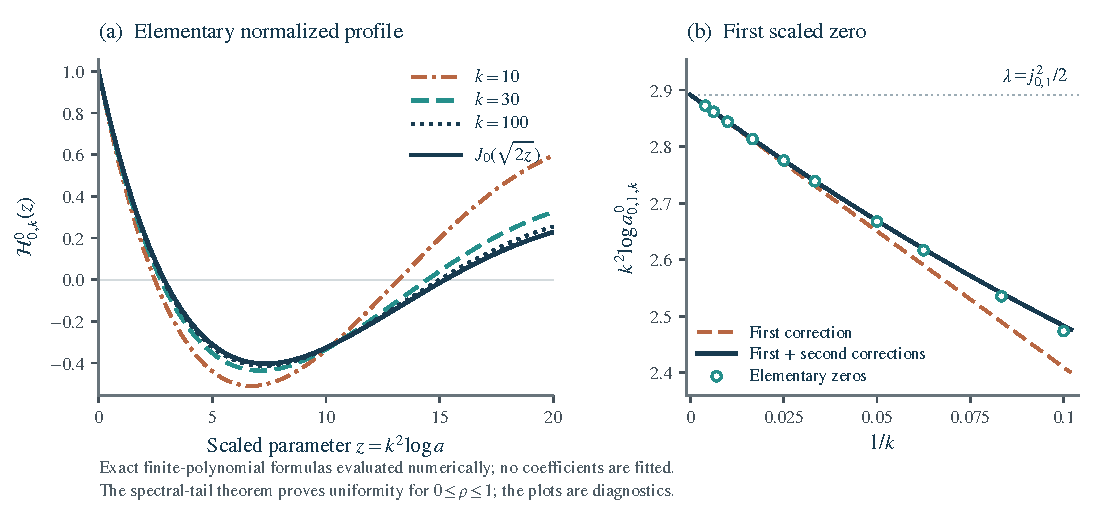
\includegraphics[width=\linewidth]{figures/bessel_profile_and_zeros.pdf}
\caption{The adjacent-index Bessel regime at $r=0$. Left: exact elementary
profile polynomials evaluated numerically and their limiting Bessel
function. Right: the first elementary scaled zero and the proved first
two corrections. No coefficients are fitted. The uniform spectral-tail
theorem, rather than the plots, establishes the result for
$0\leq\rho\leq1$.}
\label{fig:bessel}
\end{figure}
\FloatBarrier
\section{A transition for two growing log-gamma exponents}
\label{sec:gamma}

Write $f(x)=\log\Gamma(x)$, which is positive for $0<x<1$, and extend
the reflected moments to positive real exponents:
\[
 M_{n,m}=\int_0^1 f(x)^n f(1-x)^m\,\dd x.
\]
The moments themselves, their reflection symmetry, and associated exact
identities are classical \cite{ACEKMM}. The pinned manuscript proves,
for every \emph{fixed} nonnegative integer $m$,
\begin{equation}\label{eq:fixedm}
 M_{n,m}\sim\frac{\gamma^m\Gamma(n+1)}{(m+1)^{n+1}}
 \qquad(n\longrightarrow\infty),
\end{equation}
and develops a considerably sharper fixed-$m$ theory. It explicitly leaves
simultaneous growth as a separate problem. Here we locate and resolve a
transition in which \eqref{eq:fixedm} no longer has relative error tending
to zero.

Set
\begin{equation}\label{eq:gamma-constants}
 A=\frac{\zeta(2)}{2\gamma},\qquad
 B=\frac{\zeta(3)}{3\gamma}-\frac{\zeta(2)^2}{8\gamma^2},\qquad
 C=A-\gamma.
\end{equation}
Thus $C=0.84767122475766887678956780929\ldots>0$.
Only the exact definitions enter the proofs. Positivity also follows
without decimals: $\gamma<H_5-\log5<7/10$, using the first three
positive terms of $2\operatorname{arctanh}(2/3)$ to bound $\log5$
from below, while $\zeta(2)>1>2(7/10)^2$.

\begin{theorem}[Critical reflected-moment transition]\label{thm:gamma-transition}
Let $c$ range over a fixed compact subset of $\mathbb R$. As $m$ tends
to infinity through positive real values, put
\[
 L=\log m+c,\qquad q=e^{-c},\qquad n=(m+1)L.
\]
Then, uniformly in $c$,
\begin{equation}\label{eq:gamma-transition}
 \frac{(m+1)^{n+1}M_{n,m}}{\gamma^m\Gamma(n+1)}
 =e^{Cq}\left\{1+\frac{P_1(L,q)}m
       +O\!\left(\frac{L^2}{m^2}\right)\right\},
\end{equation}
where
\begin{equation}\label{eq:gamma-P1}
 P_1(L,q)=\frac L2(Cq+C^2q^2)
             -(A+\gamma)q+(B+\gamma^2)q^2.
\end{equation}
In particular, if integer pairs $(n,m)$ satisfy
$n/(m+1)-\log m\to c$, their normalized moments converge to
$\exp(Ce^{-c})$.
\end{theorem}

For example, at $c=0$ the limiting ratio is
$e^C=2.3342046795191067941\ldots$. This is an explicit counterexample
to an unrestricted extension of \eqref{eq:fixedm} to a growing reflected
exponent. It is not a counterexample to the manuscript, which keeps $m$
fixed in that assertion.

\subsection{The exact gamma expectation}
The local series needed below follow from the usual expansion of
$\log\Gamma(1+z)$ \cite{DLMFgamma}. Define
\[
 p(x)=\log\Gamma(1+x),\qquad
 h(x)=\log\left(\frac{\log\Gamma(1-x)}{\gamma x}\right).
\]
Both are real analytic near zero, with
\begin{align}\label{eq:gamma-germs}
 p(x)&=-\gamma x+\frac{\zeta(2)}2x^2+O(x^3),\\
 h(x)&=Ax+Bx^2+O(x^3).\notag
\end{align}
Substitution $x=e^{-t}$ gives an exact identity. If $T$ has gamma
density
\begin{equation}\label{eq:gamma-density}
 \frac{(m+1)^{n+1}}{\Gamma(n+1)}t^n e^{-(m+1)t},\qquad t>0,
\end{equation}
then the left side of \eqref{eq:gamma-transition} is
\begin{equation}\label{eq:gamma-expectation}
 \E e^{H_m(T)},\qquad
 H_m(t)=n\log\left(1+\frac{p(e^{-t})}{t}\right)+mh(e^{-t}).
\end{equation}
The logarithm is real: $t+p(e^{-t})=f(e^{-t})>0$.
The base approximation treats $f(e^{-t})$ as $t$ and
$f(1-e^{-t})$ as $\gamma e^{-t}$. Their first corrections act
together at the scale $me^{-L}=q$.

\begin{lemma}[Localization with the full weight]\label{lem:gamma-localization}
Fix a compact set of $c$ values and $\delta\in(0,1/2)$. Under the
hypotheses of Theorem~\ref{thm:gamma-transition}, for every fixed $N>0$,
\[
 \E\left[e^{H_m(T)}\mathbf1_{\{|T-L|>\delta\}}\right]
       =O_N(m^{-N}).
\]
The same superpolynomial bound holds for the unweighted gamma
expectations of any fixed power of $|T-L|$ on this complement.
\end{lemma}

\begin{proof}
All constants below may depend on the compact set of $c$ values and on
$\delta$. First, $p(x)<0$ for $0<x<1$: strict log-convexity of $\Gamma$
between $1$ and $2$ gives $\Gamma(1+x)<1$. Thus
\[
 e^{H_m(t)}\le e^{mh(e^{-t})}.
\]
On $t\ge L/2$, the Taylor expansion of $h$ bounds this by
$\exp(Kme^{-t})\le\exp(K'\sqrt m)$. The gamma moment-generating
function is $(1-v/(m+1))^{-(n+1)}$. Its Chernoff bounds give
\[
 \Pr(|T-L|>\delta)\le 2\exp(-c_\delta m/L)
\]
for large $m$. Since $m/L\gg\sqrt m$, the contribution of this
part of the complement is smaller than every inverse power of $m$.

Choose a fixed $\varepsilon\in(0,1/2)$. On
$\varepsilon\le t\le L/2$, $h(e^{-t})$ is bounded above by a
constant. The same gamma Chernoff calculation at $T\le L/2$ gives
$\Pr(T\le L/2)\le\exp(-c_0mL)$, with $c_0>0$; multiplying by
$e^{Km}$ preserves superpolynomial decay.

For $0<t<\varepsilon$, use the elementary endpoint bounds
\[
 f(e^{-t})\le Kt,\qquad
 f(1-e^{-t})\le D+|\log t|,
\]
with fixed positive $K,D$. The contribution before normalization is
at most
\[
 K^n\int_0^\varepsilon t^n(D-\log t)^m\,\dd t
 \le\frac{K^nD^m}{n+1-m/D}.
\]
Here $(D+y)^m\le D^m e^{my/D}$ was used, and the denominator is
positive for large $m$. Stirling's estimate shows that division by
$\gamma^m\Gamma(n+1)/(m+1)^{n+1}$ makes the logarithm of this
bound at most $-n\log L+O(n+m)$. This again is smaller than every
inverse power. The unweighted polynomial-tail assertions follow
from the same gamma bounds, or from their moment-generating
function after a fixed small exponential tilt.
\end{proof}

\subsection{Proof of the transition and its first correction}
\begin{proof}[Proof of Theorem~\ref{thm:gamma-transition}]
Put $U=T-L$. Its first raw moments about $L$, directly from
\eqref{eq:gamma-density}, are
\begin{align}\label{eq:gamma-central}
 \E U&=\frac1{m+1},&
 \E U^2&=\frac{L}{m+1}+\frac2{(m+1)^2},\\
 \E U^3&=\frac{5L}{(m+1)^2}+\frac6{(m+1)^3},&
 \E U^4&=O(L^2/m^2).\notag
\end{align}
The coefficient $5$ in the third raw moment includes the shift
between $L$ and the mean $L+1/(m+1)$.

On $|u|\le\delta$, the functions $e^{H_m(L+u)}$ and their first
four derivatives are uniformly bounded. Indeed $e^{-L}=q/m$,
$L/(L+u)$ is bounded, and the germs in \eqref{eq:gamma-germs}
can be differentiated uniformly there. To leading order write
\[
 H_0(u)=q e^{-u}\left(A-\frac{\gamma L}{L+u}\right).
\]
The values required through order $m^{-1}$ are
\begin{align}\label{eq:gamma-local-values}
 H_m(L)&=Cq+\frac1m\left\{-\gamma q
       +q^2\left(B+\frac{\zeta(2)}2-\frac{\gamma^2}{2L}\right)\right\}
       +O(m^{-2}),\\
 H_0'(0)&=q(-C+\gamma/L),\notag\\
 H_0''(0)&=q(C-2\gamma/L-2\gamma/L^2).\notag
\end{align}
The first two derivatives of $H_m(L+u)$ differ from the corresponding
derivatives of $H_0(u)$ by $O(m^{-1})$.

Taylor-expand $e^{H_m(L+u)}$ through the cubic term, with a
uniform $O(u^4)$ remainder. Lemma~\ref{lem:gamma-localization}
permits use of the full moments \eqref{eq:gamma-central}. The cubic
contribution is $O(L/m^2)$ and the quartic remainder is
$O(L^2/m^2)$. Therefore
\begin{align*}
 e^{-Cq}\E e^{H_m(T)}
 =1+\frac1m\bigg[&-\gamma q
 +q^2\left(B+\frac{\zeta(2)}2-\frac{\gamma^2}{2L}\right)
 +H_0'(0)\\
 &+\frac L2\left\{H_0''(0)+H_0'(0)^2\right\}\bigg]
 +O(L^2/m^2).
\end{align*}
Inserting \eqref{eq:gamma-local-values} cancels every displayed
negative power of $L$. Since $\gamma A=\zeta(2)/2$, the remaining
coefficient is exactly \eqref{eq:gamma-P1}. This proves the uniform
expansion. The assertion for integer pairs follows by using their
actual $c_m=n/(m+1)-\log m$ in the uniform formula.
\end{proof}

\subsection{Higher orders and the early-pole resummation}
The proof is effective at every finite order. One expands the two
analytic germs to the required degree, expands in $u$ on the localized
interval, and uses exact gamma moments. For any fixed $R$, taking
the Taylor expansion in $u$ through degree $2R+1$ bounds its next
remainder by $O((L/m)^{R+1})$. The terms from odd moments must be
kept with their signs; replacing all of them by absolute-moment
bounds would lose powers of $m$.

There is a useful algebraic description of the first correction.
Let $p_1=-\gamma$, $p_2=\zeta(2)/2$, and $s_2=p_2+B$.
The formal early-pole coefficients are
\[
 C_j(m)=[x^j]\exp\{(m+j+1)p(x)+mh(x)\}.
\]
For fixed $j$, $C_j(m)=m^jC^j/j!+O_j(m^{j-1})$, whereas
\[
 \left(\frac{m+1}{m+j+1}\right)^{n+1}
 =\left(\frac qm\right)^j
 \left\{1+\frac{Lj^2/2-j}{m}+O_j(L^2/m^2)\right\}.
\]
Thus the leading formal resummation is
$\sum_{j\ge0}(Cq)^j/j!=e^{Cq}$. With $\mathcal D=q\partial_q$,
the next coefficient is
\begin{equation}\label{eq:gamma-operator}
 e^{Cq}P_1(L,q)=
 \left\{s_2q^2+p_1q(\mathcal D+2)
                    +\frac L2\mathcal D^2-\mathcal D\right\}e^{Cq}.
\end{equation}
This identity is checked by ordinary differentiation and provides an
independent symbolic derivation of \eqref{eq:gamma-P1}.
It is not an instruction to sum the manuscript's divergent infinite
pole series. The localization proof above controls the actual integral
and supplies the analytic justification for the displayed transition.

\subsection{Location of the transition on the integer lattice}
The scale is $m\asymp n/\log n$. More precisely, if $c$ is fixed and
$w=W(e^c(n+1))$, put $k_0=(n+1)/w$. The positive real solution of
$n=(m+1)(\log m+c)$ satisfies
\begin{equation}\label{eq:gamma-inverse}
 m=k_0-1+\frac1{2k_0(w+1)}
       +O\!\left(\frac1{k_0^2(w+1)}\right).
\end{equation}
To check this, write $k=m+1$ and expand
\[
 n=k(\log k+c)-1-\frac1{2k}+O(k^{-2}).
\]
The equation $k_0(\log k_0+c)=n+1$ and one Taylor expansion, whose
derivative is $w+1$, give \eqref{eq:gamma-inverse}. Nearest-integer
choices may then be inserted using their actual value of $c_m$.

The transition settles a concrete part of the simultaneous-exponent
problem. It does not classify the regime $m/n\to\lambda>0$, nor the
uniform least-term remainder when both $m$ and the truncation index
grow. Those require additional saddle and inverse-function estimates.

\begin{figure}[tbp]
\centering
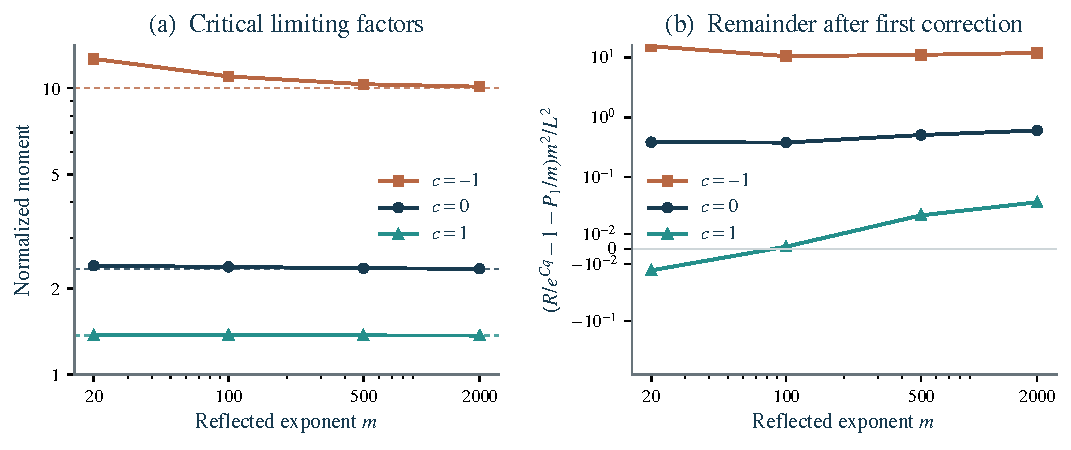
\includegraphics[width=\linewidth]{figures/gamma_transition.pdf}
\caption{Numerical diagnostics for the joint gamma-moment transition.
Left: normalized moments tend to different nonunit limits as $m$ grows.
Right: the relative error after the first correction, multiplied by
$m^2/L^2$, is consistent with the proved uniform remainder order.
The displayed values are high-precision quadrature, not interval
certificates. Six values were independently integrated in both $x$ and
$t=-\log x$.}
\label{fig:gamma}
\end{figure}
\FloatBarrier
\section{The exact reach of convergent Cayley symmetry}
\label{cayley:sec:reach}

The existing $S_4$ proof uses the involution
$\phi(t)=(1-t)/(1+t)$ together with double shuffle.  Before attempting a
larger combined relation matrix, one can answer an exact structural
question: how much does this convergent involution prove by itself, and
how much stronger does it become after all shuffle products of its
relations are admitted?  These are two different presentations.  Both
can be computed in every weight.

The resulting dimensions below are dimensions of explicitly defined
formal word quotients.  They are not dimensions of evaluated periods.
The theorem includes neither stuffle nor distribution relations, so it
does not settle the manuscript's conjectured depth-two formula for $S_6$.

\subsection{Positive forms and two commuting involutions}

Use the five formal letters
\[
 z=\frac{dt}{t},\qquad c=\frac{dt}{1-t},\qquad
 a=\frac{i\,dt}{1-it},\qquad
 b=-\frac{dt}{1+t},\qquad
 \bar a=-\frac{i\,dt}{1+it}.
\]
Letters stand both for these forms and for a basis of a rational vector
space $V$.  Let $H(w)$ denote their outer-letter-first iterated integral
from zero to one.  An admissible nonempty word has first letter different
from $c$ and last letter different from $z$.  Each such integral is
absolutely convergent: the last-letter condition controls zero, and the
first-letter condition controls one.  The other endpoint singularities
are logarithmic and integrable.

Define the letter map $\tau=-\phi^*$ by
\begin{equation}\label{cayley:eq:tau}
\begin{array}{c|ccccc}
v&z&c&a&b&\bar a\\ \hline
\tau(v)&c-b&z+b&b-\bar a&b&b-a .
\end{array}
\end{equation}
Put
\[
 C(v_1\cdots v_n)=\tau(v_n)\cdots\tau(v_1),
 \qquad
 K(z)=z,\quad K(c)=c,\quad K(b)=b,\quad K(a)=\bar a,\quad K(\bar a)=a.
\]
Here products inside a word are concatenations; linear combinations are
expanded multilinearly.  Directly from the table,
\[
 C^2=K^2=1,\qquad CK=KC.
\]
Moreover $C$ preserves admissibility.  Indeed $\tau$ maps the span of
$\{z,a,b,\bar a\}$ to the span of $\{c,a,b,\bar a\}$ and maps the latter
span back to the former.

Changing variables and reversing the integration simplex gives
\begin{equation}\label{cayley:eq:period-law}
 H(w)=H(Cw)
\end{equation}
for every admissible word.  The sign from reversing the integration path
is included in the definition $\tau=-\phi^*$.  Thus there is no omitted
weight-dependent sign in \eqref{cayley:eq:period-law}.  Conjugation gives
$H(Kw)=\overline{H(w)}$.

Let $\mathcal A_n$ be the rational span of admissible words of length $n$,
and put $\mathcal A_0=\mathbb Q$.  Superscripts $+$ and $-$ on these spaces
will mean the $+1$ and $-1$ eigenspaces of $K$.  The minus space encodes
imaginary parts; choosing one word from each nontrivial conjugate pair is
an equivalent coordinate convention.

\subsection{All-weight rank of the unmultiplied Cayley rows}

\begin{theorem}[Raw convergent Cayley rank]\label{cayley:thm:raw}
For $n\ge2$,
\[
 d_n:=\dim_{\mathbb Q}\mathcal A_n^-
 =8\cdot5^{n-2}-2\cdot3^{n-2}.
\]
The span of the imaginary projections of all weight-$n$ rows $w-Cw$
has rank
\begin{equation}\label{cayley:eq:raw-rank}
 r_n=
 \begin{cases}
 4\cdot5^{n-2}-3^{n-2},&n\text{ even},\\[2mm]
 4\cdot5^{n-2}-3^{n-2}-2\cdot5^{(n-3)/2},&n\text{ odd}.
 \end{cases}
\end{equation}
At $n=1$, the imaginary space has dimension one and the rank is zero.
\end{theorem}

\begin{proof}
For $n\ge2$, write
\[
 U=\operatorname{span}\{z,a,b,\bar a\},\qquad
 E=\operatorname{span}\{c,a,b,\bar a\}.
\]
Then $\mathcal A_n=U\otimes V^{\otimes(n-2)}\otimes E$.
The dimensions of $U,E,V$ are $4,4,5$ and their conjugation traces
are $2,2,3$.  Therefore
\[
 \dim\mathcal A_n=16\cdot5^{n-2},\qquad
 \operatorname{tr}(K\mid\mathcal A_n)=4\cdot3^{n-2},
\]
which proves the formula for $d_n$.

It remains to compute traces of reversal.  For maps $T:U\to E$ and
$S:E\to U$, the map $u\otimes e\mapsto Se\otimes Tu$ has trace
$\operatorname{tr}(ST)$.  Applied to an endpoint pair of $C$, this
trace is four, because $\tau^2=1$.  Each paired pair of internal letters
contributes five.  The same facts hold for $CK$, because $(\tau K)^2=1$.
Finally the table gives
\[
 \operatorname{tr}(\tau\mid V)=1,\qquad
 \operatorname{tr}(\tau K\mid V)=-1.
\]
Thus, for $m\ge1$,
\[
\begin{array}{c|cc}
n&\operatorname{tr}C&\operatorname{tr}CK\\ \hline
2m&4\cdot5^{m-1}&4\cdot5^{m-1}\\
2m+1&4\cdot5^{m-1}&-4\cdot5^{m-1}.
\end{array}
\]
Because $C$ and $K$ commute,
\[
 \operatorname{tr}(C\mid\mathcal A_n^-)
 =\tfrac12\bigl(\operatorname{tr}C-\operatorname{tr}CK\bigr).
\]
The image of $1-C$ is precisely the negative eigenspace of $C$.
Its rank on $\mathcal A_n^-$ is consequently
$\tfrac12(d_n-\operatorname{tr}(C\mid\mathcal A_n^-))$.
Substitution proves \eqref{cayley:eq:raw-rank}.  Weight one is checked
directly: $K$ negates $a-\bar a$ and $C$ fixes it.
\end{proof}

In particular, the raw weight-seven Cayley matrix has $24\,514$
imaginary coordinates and rank $12\,207$.  There remain $12\,307$
coordinates in that particular quotient.  This count is exact even
though writing and row-reducing the full matrix is unnecessary.

\subsection{Closing the relations under shuffle multiplication}

The raw row span is not the same as the shuffle ideal generated by the
rows.  For example, a product of two $C$-negative elements is
$C$-positive; it vanishes in the ideal quotient but need not belong to
the raw negative eigenspace.

Let
\[
 \mathcal A=\bigoplus_{n\ge0}\mathcal A_n
\]
with the shuffle product.  Both $C$ and $K$ are graded algebra
automorphisms: reversal preserves a shuffle, as does applying a linear
letter map.  Define the homogeneous ideal and quotient
\[
 \mathcal J=\langle f-Cf:f\in\mathcal A\rangle_{\mathrm{shuffle}},
 \qquad \mathcal B=\mathcal A/\mathcal J.
\]
Thus every shuffle multiple of every convergent Cayley row is included.
The ideal is stable under $K$.

Let
\[
 h_n=\dim\mathcal B_n,\qquad
 g_n=\operatorname{tr}(K\mid\mathcal B_n),\qquad
 H(t)=\sum_{n\ge0}h_nt^n,\qquad G(t)=\sum_{n\ge0}g_nt^n.
\]
The letter $g_n$ in this subsection is a character trace, not a
Gaussian double $g_{a,b}$.

\begin{theorem}[The full Cayley shuffle-ideal quotient]
\label{cayley:thm:ideal}
The algebra $\mathcal B$ is a polynomial algebra on homogeneous
generators.  Its Hilbert and conjugation-character series are the unique
formal power series with constant term one satisfying
\begin{equation}\label{cayley:eq:hilbert}
 \frac{H(t)^2}{H(t^2)}=\frac{1-t}{1-5t},
 \qquad
 \frac{G(t)^2}{H(t^2)}
   =\frac{(1-t)^2}{(1+t)(1-3t)}.
\end{equation}
In particular,
\[
 \dim\mathcal B_n^-=\frac{h_n-g_n}{2},
 \qquad
 \dim\mathcal B_n^+=\frac{h_n+g_n}{2}.
\]
An explicit product form is
\begin{equation}\label{cayley:eq:dyadic-product}
 H(t)=\prod_{j\ge0}
 \left(\frac{1-t^{2^j}}{1-5t^{2^j}}\right)^{1/2^{j+1}},
\end{equation}
where each root is expanded with constant term one.
\end{theorem}

\begin{proof}
We supply the algebraic details, including the endpoint adjustment.
Let $\widetilde{\mathcal A}$ be the full shuffle algebra on $V$,
including words that are not admissible.  This is used only as a formal
algebra in the argument.

The shuffle polynomial theorem says that the Lyndon words freely
generate $\widetilde{\mathcal A}$ over $\mathbb Q$
\cite{cayley:radford,cayley:melancon-reutenauer}.
Use the alphabet order $z<a<b<\bar a<c$.  Every Lyndon word of length
at least two is admissible: it cannot begin with the greatest letter
$c$, or end with the least letter $z$.  Conversely, the nonincreasing
Lyndon factorization of an admissible word contains neither a
one-letter factor $c$ at the beginning nor a one-letter factor $z$
at the end.  The usual triangular shuffle factorization therefore
gives
\begin{equation}\label{cayley:eq:polynomial-endpoints}
 \widetilde{\mathcal A}\simeq\mathcal A[z,c]
\end{equation}
as graded polynomial algebras.  In particular $\mathcal A$ itself is
polynomial, and its indecomposables agree with those of
$\widetilde{\mathcal A}$ in every degree at least two.

For a connected graded algebra write
$Q(\mathcal A)=\mathcal A_{>0}/(\mathcal A_{>0})^2$.
Since $C$ and $K$ are commuting involutions over $\mathbb Q$, choose
a homogeneous simultaneous eigenbasis of $Q(\mathcal A)$.
Averaging arbitrary homogeneous lifts with the four character
projectors of the group generated by $C,K$ produces simultaneous
eigenvector lifts in $\mathcal A$.  These lifts freely generate
$\mathcal A$: replacing a graded polynomial generating set by lifts
of another basis of its indecomposables is a degree-triangular
invertible change of generators.

For this generating set, $\mathcal J$ is exactly the ideal generated
by the $C$-negative generators.  One inclusion follows from
$x-Cx=2x$ for each such generator.  For the other, after all
$C$-negative generators are set to zero, $C$ acts as the identity
on every remaining polynomial.  Thus every $f-Cf$ lies in that
ideal.  Consequently $\mathcal B$ is the polynomial algebra on
the $C$-positive generators, retaining their $K$-parities.

We compute the required generator characters without constructing
the generators.  The antipode of the full shuffle Hopf algebra is
$S(w)=(-1)^{|w|}\operatorname{rev}(w)$, and every connected graded
Hopf antipode acts as minus the identity on indecomposables.
Hence reversal acts on degree-$n$ indecomposables as
$(-1)^{n-1}$.  Put $\theta=-\tau$, applied letterwise.  On
indecomposables of every positive degree we therefore have
\[
 C=-\theta.
\]
In particular, the $C$-positive generator space is the
$\theta$-negative generator space, with the same $K$-characters.

Temporarily work in the full shuffle algebra.  Let $P(t)$ be the
Hilbert series of the polynomial algebra on its $C$-positive
generators, and $Q(t)$ the corresponding $K$-trace series.
The letter traces are
\[
\begin{array}{c|rrrr}
\sigma&1&\theta&K&K\theta\\ \hline
\operatorname{tr}(\sigma\mid V)&5&-1&3&1 .
\end{array}
\]
Since the degree-$n$ word space is $V^{\otimes n}$, the four
full-shuffle character series are respectively
\[
 \frac1{1-5t},\qquad\frac1{1+t},\qquad
 \frac1{1-3t},\qquad\frac1{1-t}.
\]

A $\theta$-negative polynomial generator of degree $n$ contributes
$(1+t^n)/(1-t^n)$ to the ratio of the identity-character series
to the $\theta$-character series.  Taking the product over all
such generators gives
\[
 \frac{P(t)^2}{P(t^2)}=\frac{1+t}{1-5t}.
\]
If the same generator has $K$-sign $\varepsilon\in\{1,-1\}$,
its contribution to the ratio of the $K$-character to the
$K\theta$-character is
$(1+\varepsilon t^n)/(1-\varepsilon t^n)$.
Since $\varepsilon^2=1$, this gives
\[
 \frac{Q(t)^2}{P(t^2)}=\frac{1-t}{1-3t}.
\]
These character products are valid for an infinite generating
set, since only finitely many generators contribute to any fixed
weight.

Finally, \eqref{cayley:eq:polynomial-endpoints} removes two
degree-one indecomposables and none in higher degree.
On their quotient space, $C$ interchanges $z$ and $c$ modulo
$\mathcal A_1$, while $K$ is the identity.  Exactly one removed
generator is $C$-positive, and it is $K$-positive.  Therefore
\[
 H(t)=(1-t)P(t),\qquad G(t)=(1-t)Q(t).
\]
Substituting these two relations proves
\eqref{cayley:eq:hilbert}.  Coefficients are determined recursively
because the coefficient of the new $h_n$ or $g_n$ in its square
is two.  Iterating the first equation proves
\eqref{cayley:eq:dyadic-product} in the $t$-adic topology.
\end{proof}

The first coefficients and their interpretation are
\[
\begin{array}{c|rrrrrrr}
n&1&2&3&4&5&6&7\\ \hline
\dim\mathcal A_n^-&1&6&34&182&946&4838&24514\\
r_n&0&3&15&91&463&2419&12207\\
h_n&2&9&36&162&720&3312&15336\\
g_n&0&3&4&18&36&124&300\\
\dim\mathcal B_n^-&1&3&16&72&342&1594&7518\\
\dim\mathcal J_n^-&0&3&18&110&604&3244&16996
\end{array}
\]
At weight seven, shuffle multiplication supplies $4789$ additional
imaginary relation directions beyond the raw Cayley row span.
The remaining $7518$ coordinates are independent only in this
specified formal quotient.  Adding double shuffle can reduce it
further; the dimension of an intersection of relation spaces is not
obtained by adding their separate ranks.

\subsection{Asymptotic size and the conjugation imbalance}

\begin{corollary}[Two distinct exponential scales]
\label{cayley:cor:asymptotic}
As $n\to\infty$,
\begin{align}
 h_n&=
 \sqrt{\frac{4H(1/25)}{5\pi}}\,
 \frac{5^n}{\sqrt n}\left(1+O(n^{-1})\right),\\
 g_n&=
 \sqrt{\frac{H(1/9)}{3\pi}}\,
 \frac{3^n}{\sqrt n}\left(1+O(n^{-1})\right),\\
 \dim\mathcal B_n^-&=
 \sqrt{\frac{H(1/25)}{5\pi}}\,
 \frac{5^n}{\sqrt n}\left(1+O(n^{-1})\right).
\end{align}
Both of the first two expansions admit all orders in $1/n$.
More precisely, the relative difference between the real and
imaginary dimensions satisfies
\[
 \frac{\dim\mathcal B_n^+-\dim\mathcal B_n^-}
      {\dim\mathcal B_n^++\dim\mathcal B_n^-}
 =
 \sqrt{\frac{5H(1/9)}{12H(1/25)}}\,
 \left(\frac35\right)^n\left(1+O(n^{-1})\right).
\]
\end{corollary}

\begin{proof}
The product \eqref{cayley:eq:dyadic-product} is convergent and
nonvanishing in $|t|<1/5$.  The functional equations give
\[
 H(t)=F(t)(1-5t)^{-1/2},\qquad
 F(t)=\sqrt{(1-t)H(t^2)},
\]
and
\[
 G(t)=E(t)(1-3t)^{-1/2},\qquad
 E(t)=(1-t)\sqrt{\frac{H(t^2)}{1+t}}.
\]
The factors $F,E$ are analytic on the disk $|t|<1/\sqrt5$;
the roots are the analytic roots taking value one at zero.
Consequently the only dominant singularity for $H$ is $1/5$,
and that for $G$ is $1/3$.  The standard binomial coefficient
asymptotic
$[t^n](1-\lambda t)^{-1/2}
=\lambda^n(\pi n)^{-1/2}(1+O(n^{-1}))$,
together with Taylor expansion of the analytic factor at the
singularity, yields the first two assertions.  The factor values are
\[
 F(1/5)=\sqrt{\tfrac45 H(1/25)},\qquad
 E(1/3)=\sqrt{\tfrac13 H(1/9)}.
\]
The same Taylor expansion gives every further inverse-power
coefficient.  Finally
$\dim\mathcal B_n^\pm=(h_n\pm g_n)/2$ and division proves the ratio.
In particular, the $3^n$ character contribution is not absorbed into
an assertion that a finite $5^n/n$ expansion resolves exponentially
smaller terms: it has its own independently defined series $G$.
\end{proof}

\subsection{A completely explicit Cayley family containing \texorpdfstring{$S_6$}{S6}}

Retain
$S_p=\sum_{n\ge0}(-1)^nH_n/(2n+1)^p$.
The harmonic parity split and the positive-form convention give
\[
 S_p=\operatorname{Im}H\bigl(z^{p-1}a(a+\bar a)\bigr).
\]
This follows absolutely for $p>1$, and by a radial Abel limit for
$p=1$.

\begin{proposition}[An all-index pure-depth representation]
\label{cayley:prop:harmonic}
For every integer $p\ge1$,
\begin{equation}\label{cayley:eq:harmonic}
 S_p=\operatorname{Im}H\left((2ba-aa+a\bar a)(c-b)^{p-1}\right).
\end{equation}
All products and powers inside $H$ are concatenations.
The expanded right side contains exactly $3\cdot2^{p-1}$
admissible words, each of weight and series depth $p+1$.
In particular
\[
 \boxed{\quad
 S_6=\operatorname{Im}H\left((2ba-aa+a\bar a)(c-b)^5\right).
 \quad}
\]
\end{proposition}

\begin{proof}
Cayley transport gives
\[
 C\bigl(z^{p-1}a(a+\bar a)\bigr)
 =(2b-a-\bar a)(b-\bar a)(c-b)^{p-1}.
\]
Both $2b-a-\bar a$ and $c-b$ are fixed by conjugation.
Taking half the difference with the conjugate and then grouping
the three conjugate pairs gives exactly the imaginary part in
\eqref{cayley:eq:harmonic}.  The first letters in the resulting
three word families are $a$ or $b$, and all letters are nonzero
kernel letters.  Thus every expanded word is admissible and
represents an all-one colored multiple polylogarithm.
\end{proof}

This proposition provides a new explicit high-depth expression
and a compact formal certificate for the weight-seven mixed sum.
It does not turn the manuscript's proposed depth-two $S_6$
reduction into a theorem.  The latter still requires an exact
combination of additional relations.

For a real-integral check of conventions, the same identity yields
\[
 S_p=\frac1{(p-1)!}\int_0^1
 \log^{p-1}\!\left(\frac{1+u}{1-u}\right)
 \frac{\log\!\left((1+u)^2/(2(1+u^2))\right)}{1+u^2}\,du.
\]
Indeed the iterated integral of $(c-b)^{p-1}$ up to $u$ is the
displayed logarithmic power divided by $(p-1)!$.
Integrating the two outer letters in
$2ba-aa+a\bar a$, and taking imaginary parts, produces the
remaining kernel.  The substitution $u=(1-x)/(1+x)$ returns
the original Mellin representation of $S_p$.

There is also a direct verification of this real integral, independent
of the word expansion.  Start from the already convergent identity
\[
 S_p=-\frac1{(p-1)!}\int_0^1
 (-\log x)^{p-1}\frac{\log(1+x^2)}{1+x^2}\,dx.
\]
With $x=(1-u)/(1+u)$ the endpoint pair $(0,1)$ becomes $(1,0)$, and
\[
 -\log x=\log\frac{1+u}{1-u},\qquad
 \frac{dx}{1+x^2}=-\frac{du}{1+u^2},\qquad
 \log(1+x^2)=-\log\frac{(1+u)^2}{2(1+u^2)}.
\]
Substitution, including the reversed integration limits, gives the
displayed formula.  Near $u=1$ the new logarithmic kernel vanishes
quadratically in $1-u$, so every fixed logarithmic power remains
integrable.  At $u=0$ the integrand is bounded (and has a zero of
order $p-1$ when $p>1$).

\subsection{Finite verification and the remaining mixed reduction}

The supplied program \texttt{check\_cayley\_ranks.py} is independent
of the older report's word implementation.  It builds all admissible
words, expands the displayed letter transformation, checks $C^2=1$
and $CK=KC$, and computes rational ranks by integer elimination
with gcd normalization.  It also constructs every shuffle lift
$H(v)H(w-Cw)$ with total weight at most four.

The exact matrix results are
\[
\begin{array}{c|rrrr}
n&1&2&3&4\\ \hline
\dim\mathcal A_n&3&16&80&400\\
\text{raw full rank}&1&6&38&190\\
\text{all lifted full rank}&1&7&44&238\\
\text{raw imaginary rank}&0&3&15&91\\
\text{all lifted imaginary rank}&0&3&18&110
\end{array}
\]
The weight-four lifted calculation contains all $1136$ prescribed
row instances.  These are exact rational checks, not modular rank
estimates.  They audit the all-weight proofs; the proofs do not
depend on extrapolating the table.

The separate program \texttt{verify\_harmonic\_cayley.py} rebuilds
\eqref{cayley:eq:harmonic} for $1\le p\le8$ and obtains zero exact
residual in every case.  The file
\texttt{S6\_cayley\_depth\_seven.json} lists all $96$ terms for
$p=6$.  The verifier imports no numerical polylogarithm evaluator.

An exploratory weight-seven double-shuffle computation generated
$51\,244$ normalized rows, in addition to a selected Cayley row.
The sparse search was stopped after substantial fill-in; it
produced neither an exact certificate for the conjectured $S_6$
formula nor a separating functional.  No membership or
nonmembership claim follows from that unfinished computation.
The exact quotient and rank theorems above concern the fully
specified Cayley-only presentations and remain unaffected.

\section{Verification, correction proposals, and integration}
\label{sec:verification}

\subsection{What the computations establish}
The proof-bearing arithmetic uses exact integers, rational intervals,
or rational polynomial identities. The analytic theorems additionally
require the convergence, sign-change, localization, and asymptotic
arguments written in the preceding sections. The code is not a substitute
for those arguments and is not a proof-assistant formalization.

The included exact replays cover:
\begin{enumerate}
\item the two Bernstein positivity certificates, their substitutions,
the local angular coefficient, and the rational inequalities in the
normalized-radius proof;
\item outward-rounded rational certificates for two fractional
thresholds, opposite quartic signs, and the local maximum and minimum
scaling prefactors;
\item exact shifted gamma moments and two independent symbolic
derivations of the transition's first correction;
\item 48 rational sign enclosures for $f_{n,k}(2)$ and the elementary
logarithm bounds used in the spectral-tail estimate;
\item exact Faulhaber generation of Bessel profile operators and simple
zero coefficients through four inverse powers of $k$ in the scaled
variable;
\item all raw and shuffle-lifted Cayley matrices through weight four,
including every one of the 1136 prescribed lifted row instances at
weight four;
\item exact zero residuals for the explicit $S_p$ Cayley expression for
$1\le p\le8$, together with the full 96-term expansion at $p=6$.
\end{enumerate}

The separate diagnostic files contain 24 regularized moment comparisons,
22 endpoint-scale examples, five angular roots, 30 elementary Bessel-zero
comparisons, six full-Lerch comparisons, and 12 reflected-moment
quadratures. Six of the latter are computed in both original and
logarithmic coordinates. The kernel calculations use 80 decimal digits;
the Bessel comparisons use 250; the gamma quadratures use 65.
The precision and the interpretation of each table are stored with it.
These numbers are diagnostic precision settings, not certified error
estimates for every displayed decimal.

\subsection{The existing conjectures and their current status}
The local normalized-radius question is resolved by
Theorem~\ref{thm:radius-local-sign}. The global-radius claim for the stated integer range remains
open. Theorems~\ref{turn:thm:maximum} and \ref{turn:thm:minimum}
prove that a blanket fractional extension fails. In particular, a sign in a Taylor expansion near zero does not
prove monotonicity on the complete radius interval.

For clarity, one frozen form of the manuscript's $S_6$ conjecture is
\begin{align}\label{eq:S6-open}
 S_6\stackrel{?}{={}}&
 \frac{722}{527}g_{6,1}+\frac{40}{527}g_{4,3}
 -\frac{128}{155}g_{2,5}
 +\frac{15191}{28569600}\pi^7\notag\\
 &-\frac3{124}\beta(2)\zeta(5)
 -\frac{2373}{10540}\beta(4)\zeta(3)
 -2\beta(6)\log2.
\end{align}
The source already contains a rigorous very small residual enclosure
and proves equivalence with another proposed basket. Neither fact
establishes equality. Proposition~\ref{cayley:prop:harmonic} gives an
exact expression of larger depth, while Theorem~\ref{cayley:thm:ideal}
identifies an entire symmetry quotient. Neither closes the remaining
double-shuffle reduction in \eqref{eq:S6-open}.

\subsection{Corrections that are justified, and claims that should not be changed}
The audit did not find a newly verified false theorem in the canonical
portions used here. It did identify stale statements in historical
reports, and the extension work exposes several places where a proposed
broader statement would be false or unjustified. The integration ledger
records these separately.

\paragraph{Stale $S_4$ status.}
The pending Lerch report's attribution paragraph still says that it does
not resolve the mixed $S_4$ conjecture. As a statement about that report's
own contribution this is harmless, but as a current-status description
it is obsolete. An editorial annotation should say: ``The canonical
manuscript now proves $S_4$ by an exact convergent Cayley and
double-shuffle certificate; the mixed $S_6$ reduction remains
conjectural.'' Historical source packages can be retained unchanged,
with the annotation in their integration record.

\paragraph{Critical endpoint atoms.}
When extending the signed kernel to $a+b=1$, the term containing
$1/\Gamma(a+b-1)$ cannot simply be deleted. The family
$e^{-T}T^{\varepsilon-1}/\Gamma(\varepsilon)$ tends weakly to an
atom at $T=0$. Omitting it loses mass $(1-b)^{-1}$ and violates
even the zeroth moment. Theorem~\ref{subunit:thm:domain} gives the
correct measure statement and normalization. This is a correction to
the naive extension, not to the earlier theorem for $a\ge1$.

\paragraph{Boundary Fourier language.}
In the atomic cases $A_n$ tends to a nonzero constant, so the complex
Fourier terms $A_ne^{in\theta}$ do not tend to zero. The correct
unit-circle interpretation is the Abel value of the analytic
continuation. Every angular theorem also concerns $0<\theta<\pi$:
the real endpoints have zero imaginary part automatically.

\paragraph{Limits of moment and zero statements.}
The fixed-reflected-exponent leading formula must retain ``$m$ fixed''.
Its unrestricted growing-$m$ extension has limiting relative factor
$e^{Ce^{-c}}$, which differs from one. Likewise, a fixed-index
Stieltjes expansion cannot be used without proof when $n\sim k$.
The Bessel theorem resolves one such new regime, and deliberately
does not supply a global count of all its positive zeros.

\paragraph{Relation spaces and numerical independence.}
The raw Cayley image and its shuffle ideal differ already in low
weights. In weight seven their imaginary ranks are respectively
12207 and 16996. Neither rank is a dimension theorem for numerical
periods, and neither can simply be added to a double-shuffle rank:
the intersection must be computed. Similarly, failure of a sparse
search to finish is neither nonmembership nor a separating functional.

\subsection{Reproduction and repository placement}
The proposed destination is
\codefile{Analysis/Polylogarithms/docs/reports/fractional-cayley-scaling/}.
The package is self-contained: \codefile{article.tex} inputs the
section fragments and bibliography, and the vector figures are already
included. The exact replay command is
\begin{quote}\ttfamily
python3 code/run\_verification.py
\end{quote}
Adding \codefile{--diagnostics} repeats the slower numerical checks.
The coefficient and matrix programs can also be run separately.
The \codefile{Makefile} builds the PDF using \codefile{latexmk};
\codefile{code/build_pdf.py} supplies a simple multi-pass fallback.
The machine-readable verification report records exit statuses,
software versions, and the scope of each job.

\codefile{integration/INTEGRATION.md} maps new results to the existing
chapters and distinguishes completed, partially resolved, and open
items. \codefile{integration/source_snapshot.json} records the pinned
revision and hashes of the source files used in the audit.
\codefile{MANIFEST.sha256} covers the delivered files. The large
unfinished $S_6$ matrices and retrieved historical report copies are
excluded; the new reproducible results do not depend on them.

\section{Further research questions and proposed programme}
\label{sec:agenda}

The following questions are concrete continuations of the proved
results. Each item identifies the missing mathematical step, so that a
future finite experiment can be judged against a defined goal.

\subsection{Angular geometry and fractional kernels}

\paragraph{1. Complete the original global normalized-radius conjecture.}
Prove or refute that $\eta_{a,b}(\rho)$ decreases on $(0,1]$ for
every integer $a\ge2,b>0$, and establish the proposed $a=1$
trichotomy. Theorem~\ref{thm:radius-local-sign} removes the first local
obstruction. A useful next step is an exact sign formula for
$\partial_\rho\eta$ evaluated at its implicit zero, followed by a
variation-diminishing or ordered-kernel argument. A proof must control
the moving zero, not merely the integrand at a fixed angle.

\paragraph{2. Classify fractional radial turning points.}
For $0<b<1$, the curve $a_*(b)$ determines the local quadratic
coefficient. Theorems~\ref{turn:thm:maximum} and \ref{turn:thm:minimum}
prove opposite local bifurcations on this curve, so the quartic sign
is not constant. Determine the number of zeros of
$Q(a_*(b),b)$, certify the diagnostic crossing near
$b=0.9974937898734204$, and analyze the sixth-order coefficient there.
This is a specific candidate for a higher-order radial transition.
Determine also whether a single global radial curve can have several
turning points; the local theorems do not exclude that possibility.

\paragraph{3. Determine the complex zero region below the moment boundary.}
The finite signed-measure classification is sharp, but it does not
classify all parameters for complex nonvanishing. For $a=0$,
$F_{0,b}(z)=z\Li_b(z)/(1-z)$ gives a different route. Determine
whether nonzero complex zeros appear for $0<a<1-b$, and, if they do,
locate the first parameter boundary. A generalized Stieltjes transform
or a distributional moment representation may replace finite variation;
it would require a new zero argument.

\paragraph{4. Resolve the two-parameter corner $a\downarrow0,b\to1$.}
For fixed $b\ne1$ the crossing approaches one by a power law, while at
$b=1$ its distance is essentially $e^{-1/a}$. Derive a uniform
interpolation when $b-1$ and $a$ vanish together. The exact rescaled
kernel is a useful starting point, but neither fixed-$b$ asymptotic
is uniform at this corner. Determine the corresponding total-variation
profile and the weak limits after renormalization.

\paragraph{5. Optimize the Euler constant in the extended domain.}
The constants $(1-b)^{-1}$, $\zeta(b)$ and
$e^{a(\gamma+\psi(a))}/(a^2\Gamma(a))$ give explicit enclosures.
They are not claimed to be optimal remainder constants. Characterize
the exact signed mass as a function of $(a,b)$, sharpen the remainder
using its vanishing moments, and design an interval evaluator that
remains effective as the positive density collapses into an atom.

\subsection{Lerch zeros and overlapping asymptotic regimes}

\paragraph{6. Unfold the central Bessel zero.}
For fixed $r>0$, $\Psi_r$ has a multiple zero at zero. Its splitting
depends on a spectral contribution that is invisible to every algebraic
order in $1/k$. Obtain its leading exponential scale and sign, including
possible cancellation among shifted terms. This should connect the
fixed-$(n,k)$ small-$\rho$ Puiseux theorem with the joint limit
$n=k+r$, but the limits need not commute.

\paragraph{7. Allow the Bessel order or zero label to grow.}
Determine a range of $r=r(k)$ and $m=m(k)$ in which the fixed-order
Bessel approximation is still uniform. Find the transition to an
appropriate large-order or turning-point profile. The first technical
obligation is a uniform coefficient bound for the symmetric product
after the factorial transform, rather than a fixed-$r$ formal expansion.

\paragraph{8. Sharpen the exponential Lerch deformation.}
The factor $e^{-k/20}$ is explicit and adequate for separation of
scales, but it is deliberately conservative. Optimize the coefficient
contour and derive the actual leading exponential term, including its
oscillatory sign. This would explain the changes of sign seen in the
full-Lerch diagnostics and quantify when the first shift dominates.

\paragraph{9. Determine the sign pattern of $f_{n,k}(2)$.}
The all-pair small-$\rho$ theorem reduces the remaining count choice
to a nonzero integer polynomial evaluated at $\log2$. Find a useful
closed sign criterion in large regions of the $(n,k)$ lattice, or an
asymptotic sign law when both indices grow. Transcendence proves
nonvanishing, but supplies no practical separation bound. Rational
interval certificates can produce a reliable initial map.

\subsection{Reflected moments and uniform asymptotics}

\paragraph{10. Extend the critical transition to complete finite orders.}
The gamma localization argument and exact moments give an algorithm
for higher terms. Compute and prove a useful recurrence for the
coefficient functions beyond $P_1$, determine whether all negative
powers of $L$ cancel, and produce explicit computable remainder
constants on prescribed compact $c$ intervals. The first cancellation
is proved here; a general cancellation pattern needs its own argument.

\paragraph{11. Treat proportional growth and symmetry of the saddle.}
For $m/n\to\lambda>0$, analyze the critical points of
\[
 \log\log\Gamma(x)+\lambda\log\log\Gamma(1-x).
\]
Prove uniqueness or classify competing maxima, obtain a uniform
Laplace expansion, and connect it to the $m\asymp n/\log n$
boundary regime. The exact symmetry $M_{n,m}=M_{m,n}$ is an
essential consistency test. Numerical maximization alone cannot
exclude an additional saddle.

\paragraph{12. Make optimal truncation uniform in the reflected exponent.}
The source's sharp fixed-$m$ remainder is a separate theorem from the
present joint transition. Determine a common range in $(n,m,N)$ for
which late inverse-function coefficients and the least-term remainder
are uniform. The early-pole resummation suggests the correct matching,
but does not license summation of a divergent infinite pole series.

\subsection{Formal relation quotients and special values}

\paragraph{13. Prove the frozen $S_6$ depth-two formula.}
Construct simultaneous Cayley and conjugation eigenvector generators,
reduce the weight-seven problem to the 7518-dimensional imaginary
Cayley quotient, and impose double shuffle there with exact lifting
data. A successful output is a rational certificate whose expanded
residual is exactly zero. A negative answer for a specified presentation
requires a separating functional; it does not disprove the numerical
identity unless the presentation is known to be complete.

\paragraph{14. Determine the intersection with double shuffle.}
Theorem~\ref{cayley:thm:ideal} answers the Cayley-only problem in all
weights. Find the Hilbert or character series after adding a precisely
specified regularized double-shuffle ideal. Compare raw rows,
multiplicative closures, distribution, and rational pullback relations.
Any dimension conjecture should specify which algebra and which ideal
are meant, and should distinguish formal dimensions from periods.

\paragraph{15. Generalize the involution quotient theorem.}
The proof uses a graded polynomial shuffle algebra, two commuting
involutions, and a finite endpoint correction. Extend it to other
root-of-unity alphabets and rational changes of variables when the
admissible subalgebra is stable. Determine which transformations can be
simultaneously linearized on generators and what replaces the dyadic
functional equation when the acting symmetry has higher order.

\paragraph{16. Search for short consequences of the explicit $S_p$ family.}
The all-depth expression is exact but expands exponentially. Seek
families in which conjugation, parity, or shuffle symmetries collapse
most terms, and identify weights where a depth-two basket can plausibly
be complete. Freeze each candidate basket and coefficient vector before
verification, retain exact residual enclosures, and then seek symbolic
proofs. The rejected earlier $S_8$ vector should remain a regression
case rather than being silently replaced.

\subsection{Suggested order of work}
The most immediate finite task is the equivariant Cayley reduction for
$S_6$, because the quotient theorem gives a concrete smaller target.
On the analytic side, the global integer-order radial conjecture and
the two-parameter kernel corner are natural next goals: the present
sign and scaling formulas expose their remaining obstacles. The central
Bessel unfolding and uniform late-term gamma theory are more demanding
matching problems. All four directions benefit from keeping exact
finite verification separate from conjectural global extrapolation.

\clearpage
\begin{thebibliography}{99}

\bibitem{ProveIt}
V.~Reshetnikov and contributors,
\emph{ProveIt: Polylogarithms manuscript}, source snapshot
\baseline, inspected 10 October 2026.
\url{https://github.com/VladimirReshetnikov/ProveIt/tree/28357e8ca63dd78327db91d9be239d75e4462879/Analysis/Polylogarithms/docs/manuscript}.
Relevant chapters include signed kernels, cyclotomic quotients,
reflected moments, and Stieltjes zero geometry.

\bibitem{AngularBaseline}
\repo\ research reports,
\emph{Angular Zero Continuation}, source at the same pinned revision,
\codefile{docs/reports/angular-zero-continuation/article.tex}.
\url{https://github.com/VladimirReshetnikov/ProveIt/blob/28357e8ca63dd78327db91d9be239d75e4462879/Analysis/Polylogarithms/docs/reports/angular-zero-continuation/article.tex}.

\bibitem{LerchBaseline}
\repo\ research reports,
\emph{Lerch Endpoint Singularities and Stieltjes Zero Bifurcations},
source at the same pinned revision,
\codefile{docs/reports/lerch-zero-bifurcations/article/lerch_zero_bifurcations.tex}.
\url{https://github.com/VladimirReshetnikov/ProveIt/blob/28357e8ca63dd78327db91d9be239d75e4462879/Analysis/Polylogarithms/docs/reports/lerch-zero-bifurcations/article/lerch_zero_bifurcations.tex}.

\bibitem{CayleyBaseline}
\repo\ research reports,
\emph{Cayley $S_4$ Continuation}, source package at the same pinned
revision, \codefile{docs/reports/cayley-s4-continuation/}.
\url{https://github.com/VladimirReshetnikov/ProveIt/tree/28357e8ca63dd78327db91d9be239d75e4462879/Analysis/Polylogarithms/docs/reports/cayley-s4-continuation}.

\bibitem{DLMFhurwitz}
NIST Digital Library of Mathematical Functions,
\emph{\S25.11: Hurwitz zeta function}, especially 25.11.4 and
25.11.25. \url{https://dlmf.nist.gov/25.11}.

\bibitem{DLMFdigamma}
NIST Digital Library of Mathematical Functions,
\emph{\S5.9: Integral representations}, especially 5.9.13.
\url{https://dlmf.nist.gov/5.9}.

\bibitem{DLMFgamma}
NIST Digital Library of Mathematical Functions,
\emph{\S5.7: Series expansions of the gamma and psi functions}.
\url{https://dlmf.nist.gov/5.7}.

\bibitem{DLMFbessel}
NIST Digital Library of Mathematical Functions,
\emph{\S10.2: Definitions; \S10.21: Zeros of Bessel functions}.
\url{https://dlmf.nist.gov/10.2};
\url{https://dlmf.nist.gov/10.21}.

\bibitem{Lindemann}
F.~Lindemann, \emph{Ueber die Zahl $\pi$},
Mathematische Annalen \textbf{20} (1882), 213--225.
\href{https://doi.org/10.1007/BF01446522}{doi:10.1007/BF01446522}.

\bibitem{ACEKMM}
T.~Amdeberhan, M.~W.~Coffey, O.~Espinosa, C.~Koutschan,
D.~V.~Manna and V.~H.~Moll,
\emph{Integrals of powers of loggamma},
Proceedings of the American Mathematical Society \textbf{139} (2011),
535--545.
\href{https://doi.org/10.1090/S0002-9939-2010-10589-0}{doi:10.1090/S0002-9939-2010-10589-0}.
Author manuscript: \url{https://www.math.tulane.edu/~vhm/papers_html/lg-subm.pdf}.

\bibitem{cayley:radford}
D.~E.~Radford,
\emph{A natural ring basis for the shuffle algebra and an application
to group schemes}, Journal of Algebra \textbf{58} (1979), 432--454.
\href{https://doi.org/10.1016/0021-8693(79)90171-6}{doi:10.1016/0021-8693(79)90171-6}.

\bibitem{cayley:melancon-reutenauer}
G.~Melan\c{c}on and C.~Reutenauer,
\emph{Lyndon words, free algebras and shuffles},
Canadian Journal of Mathematics \textbf{41} (1989), 577--591.
\href{https://doi.org/10.4153/CJM-1989-025-2}{doi:10.4153/CJM-1989-025-2}.

\bibitem{ZhaoOctahedral}
J.~Zhao, \emph{Multiple polylogarithm values at roots of unity},
Comptes Rendus Math\'ematique \textbf{346} (2008), 1029--1032;
expanded version arXiv:0810.1064.
\url{https://arxiv.org/abs/0810.1064}.

\end{thebibliography}

\end{document}
